%
% file: localoperator.tex
% author: Victor Brena
% description: Briefly describes properties of the local operator.
%

\chapter{Appendix D: Issuer matched CBI Dataset Analysis}
\label{appD}

%%%%%%%%%%%%%%%%%%%%%%%%%%%%%%%%%%%%%%%%%%%%%%%%%%%%%%%%%%%%
\section{D.1 Descriptive Statistics}
%%%%%%%%%%%%%%%%%%%%%%%%%%%%%%%%%%%%%%%%%%%%%%%%%%%%%%%%%%%%


%%%%%%%%%%%%%%%%%%%%%%%%%%%%%%%%%%%%%%%%%%%%%%%%%%%%%%%%%%%%
\subsection{D.1.1 Summary Statistics}
%%%%%%%%%%%%%%%%%%%%%%%%%%%%%%%%%%%%%%%%%%%%%%%%%%%%%%%%%%%%


%%%%%%%%%%%%%%%%%%%%%%%%%%%%%%%%%%%%%%%%%%%%%%%%%%%%%%%%%%%%
%\subsubsection{D.1.1.1 Green Bonds}
%%%%%%%%%%%%%%%%%%%%%%%%%%%%%%%%%%%%%%%%%%%%%%%%%%%%%%%%%%%%
\begin{table}[H] \centering
  \footnotesize
  \caption{Data Matched CBI Green Bond Summary Statistics} 
  \label{desc4} 
\begin{tabular}{@{\extracolsep{5pt}}lccccccc} 
\\[-1.8ex]\hline 
\hline \\[-1.8ex] 
Statistic & \multicolumn{1}{c}{N} & \multicolumn{1}{c}{Mean} & \multicolumn{1}{c}{St. Dev.} & \multicolumn{1}{c}{Min} & \multicolumn{1}{c}{Pctl(25)} & \multicolumn{1}{c}{Pctl(75)} & \multicolumn{1}{c}{Max} \\ 
\hline \\[-1.8ex] 
Time to Maturity (Days) & 425 & 2,781.809 & 1,572.795 & 367 & 1,833 & 3,659 & 11,180 \\ 
Issue Amount & 425 & 1,192.976 & 1,731.084 & 500.000 & 564.302 & 1,120.900 & 17,377.000 \\  
Coupon Rate & 425 & 1.257 & 1.142 & 0.000 & 0.375 & 1.875 & 6.125 \\ 
Guarantor & 425 & 0.169 & 0.376 & 0 & 0 & 0 & 1 \\ 
Offer Yield to Maturity & 425 & 1.300 & 1.152 & $-$0.305 & 0.465 & 1.914 & 6.125 \\
Green Flag & 425 & 1.000 & 0.000 & 1 & 1 & 1 & 1 \\ 
2008 & 425 & 0.000 & 0.000 & 0 & 0 & 0 & 0 \\ 
2009 & 425 & 0.000 & 0.000 & 0 & 0 & 0 & 0 \\ 
2010 & 425 & 0.000 & 0.000 & 0 & 0 & 0 & 0 \\ 
2011 & 425 & 0.000 & 0.000 & 0 & 0 & 0 & 0 \\ 
2012 & 425 & 0.002 & 0.049 & 0 & 0 & 0 & 1 \\ 
2013 & 425 & 0.019 & 0.136 & 0 & 0 & 0 & 1 \\ 
2014 & 425 & 0.019 & 0.136 & 0 & 0 & 0 & 1 \\ 
2015 & 425 & 0.054 & 0.227 & 0 & 0 & 0 & 1 \\ 
2016 & 425 & 0.073 & 0.260 & 0 & 0 & 0 & 1 \\ 
2017 & 425 & 0.096 & 0.296 & 0 & 0 & 0 & 1 \\ 
2018 & 425 & 0.106 & 0.308 & 0 & 0 & 0 & 1 \\ 
2019 & 425 & 0.169 & 0.376 & 0 & 0 & 0 & 1 \\ 
2020 & 425 & 0.120 & 0.325 & 0 & 0 & 0 & 1 \\ 
2021 & 425 & 0.186 & 0.389 & 0 & 0 & 0 & 1 \\ 
2022 & 425 & 0.155 & 0.363 & 0 & 0 & 0 & 1 \\ 
AAA & 425 & 0.320 & 0.467 & 0 & 0 & 1 & 1 \\ 
AA & 425 & 0.193 & 0.395 & 0 & 0 & 0 & 1 \\ 
A & 425 & 0.231 & 0.422 & 0 & 0 & 0 & 1 \\ 
BBB & 425 & 0.245 & 0.430 & 0 & 0 & 0 & 1 \\ 
BB & 425 & 0.012 & 0.108 & 0 & 0 & 0 & 1 \\ 
B & 425 & 0.000 & 0.000 & 0 & 0 & 0 & 0 \\ 
AUD & 425 & 0.007 & 0.084 & 0 & 0 & 0 & 1 \\ 
BRL & 425 & 0.000 & 0.000 & 0 & 0 & 0 & 0 \\ 
CAD & 425 & 0.024 & 0.152 & 0 & 0 & 0 & 1 \\ 
CLP & 425 & 0.000 & 0.000 & 0 & 0 & 0 & 0 \\ 
CNY & 425 & 0.002 & 0.049 & 0 & 0 & 0 & 1 \\ 
EUR & 425 & 0.666 & 0.472 & 0 & 0 & 1 & 1 \\ 
GBP & 425 & 0.016 & 0.127 & 0 & 0 & 0 & 1 \\ 
JPY & 425 & 0.002 & 0.049 & 0 & 0 & 0 & 1 \\ 
MXN & 425 & 0.000 & 0.000 & 0 & 0 & 0 & 0 \\ 
NZD & 425 & 0.000 & 0.000 & 0 & 0 & 0 & 0 \\ 
NOK & 425 & 0.002 & 0.049 & 0 & 0 & 0 & 1 \\ 
SEK & 425 & 0.014 & 0.118 & 0 & 0 & 0 & 1 \\ 
CHF & 425 & 0.000 & 0.000 & 0 & 0 & 0 & 0 \\ 
TRY & 425 & 0.000 & 0.000 & 0 & 0 & 0 & 0 \\ 
USD & 425 & 0.266 & 0.442 & 0 & 0 & 1 & 1 \\ 
\hline \\[-1.8ex] 
\end{tabular} 
\end{table} 

\newpage

\begin{table}[!htbp] \centering
  \footnotesize
  \caption{Data Matched CBI Green Bond Summary Statistics cont.} 
  \label{} 
\begin{tabular}{@{\extracolsep{5pt}}lccccccc} 
\\[-1.8ex]\hline 
\hline \\[-1.8ex] 
Statistic & \multicolumn{1}{c}{N} & \multicolumn{1}{c}{Mean} & \multicolumn{1}{c}{St. Dev.} & \multicolumn{1}{c}{Min} & \multicolumn{1}{c}{Pctl(25)} & \multicolumn{1}{c}{Pctl(75)} & \multicolumn{1}{c}{Max} \\ 
\hline \\[-1.8ex] 
Annual Coupon & 425 & 0.720 & 0.450 & 0 & 0 & 1 & 1 \\ 
Semi Annual Coupon & 425 & 0.278 & 0.448 & 0 & 0 & 1 & 1 \\ 
Quarterly & 425 & 0.000 & 0.000 & 0 & 0 & 0 & 0 \\ 
Maturity & 425 & 0.002 & 0.049 & 0 & 0 & 0 & 1 \\ 
Basic Materials & 425 & 0.007 & 0.084 & 0 & 0 & 0 & 1 \\ 
Consumer Cyclicals & 425 & 0.007 & 0.084 & 0 & 0 & 0 & 1 \\ 
Consumer Non-Cyclicals & 425 & 0.007 & 0.084 & 0 & 0 & 0 & 1 \\ 
Financials & 425 & 0.640 & 0.481 & 0 & 0 & 1 & 1 \\ 
Government Activity & 425 & 0.160 & 0.367 & 0 & 0 & 0 & 1 \\ 
Healthcare & 425 & 0.002 & 0.049 & 0 & 0 & 0 & 1 \\ 
Industrials & 425 & 0.045 & 0.207 & 0 & 0 & 0 & 1 \\ 
Institutions, Associations \& Organizations & 425 & 0.040 & 0.196 & 0 & 0 & 0 & 1 \\ 
Real Estate & 425 & 0.024 & 0.152 & 0 & 0 & 0 & 1 \\ 
Technology & 425 & 0.012 & 0.108 & 0 & 0 & 0 & 1 \\ 
Utilities & 425 & 0.056 & 0.231 & 0 & 0 & 0 & 1 \\ 
Senior Secured Mortgage & 425 & 0.092 & 0.289 & 0 & 0 & 0 & 1 \\ 
Senior Secured & 425 & 0.016 & 0.127 & 0 & 0 & 0 & 1 \\ 
Senior Unsecured & 425 & 0.673 & 0.470 & 0 & 0 & 1 & 1 \\ 
Senior Non-Preferred & 425 & 0.085 & 0.279 & 0 & 0 & 0 & 1 \\ 
Senior Preferred & 425 & 0.099 & 0.299 & 0 & 0 & 0 & 1 \\ 
Senior Subordinated Unsecured & 425 & 0.002 & 0.049 & 0 & 0 & 0 & 1 \\ 
Subordinated Unsecured & 425 & 0.007 & 0.084 & 0 & 0 & 0 & 1 \\ 
Unsecured & 425 & 0.024 & 0.152 & 0 & 0 & 0 & 1 \\ 
Public Sector & 425 & 0.372 & 0.484 & 0 & 0 & 1 & 1 \\ 
Corporate Sector & 425 & 0.628 & 0.484 & 0 & 0 & 1 & 1 \\ 
\hline \\[-1.8ex] 
\end{tabular} 
\end{table} 

%%%%%%%%%%%%%%%%%%%%%%%%%%%%%%%%%%%%%%%%%%%%%%%%%%%%%%%%%%%%
%\subsubsection{D.1.1.2 Brown Bonds}
%%%%%%%%%%%%%%%%%%%%%%%%%%%%%%%%%%%%%%%%%%%%%%%%%%%%%%%%%%%%

\begin{table}[!htbp] \centering 
  \footnotesize
  \caption{Data Matched CBI Brown Bond Summary Statistics} 
  \label{} 
\begin{tabular}{@{\extracolsep{5pt}}lccccccc} 
\\[-1.8ex]\hline 
\hline \\[-1.8ex] 
Statistic & \multicolumn{1}{c}{N} & \multicolumn{1}{c}{Mean} & \multicolumn{1}{c}{St. Dev.} & \multicolumn{1}{c}{Min} & \multicolumn{1}{c}{Pctl(25)} & \multicolumn{1}{c}{Pctl(75)} & \multicolumn{1}{c}{Max} \\ 
\hline \\[-1.8ex] 
Time to Maturity (Days) & 4,034 & 2,699.585 & 2,545.535 & 373 & 1,743 & 3,485.2 & 36,532 \\ 
Issue Amount & 4,034 & 1,694.083 & 1,649.116 & 500 & 797.6 & 1,830.8 & 30,089 \\ 
Coupon Rate & 4,034 & 2.113 & 1.588 & 0.010 & 0.875 & 3.000 & 20.000 \\ 
Guarantor & 4,034 & 0.185 & 0.388 & 0 & 0 & 0 & 1 \\ 
Offer Yield to Maturity & 4,034 & 2.143 & 1.590 & 0.003 & 0.914 & 3.040 & 20.000 \\
Green Flag & 4,034 & 0.000 & 0.000 & 0 & 0 & 0 & 0 \\ 
2008 & 4,034 & 0.048 & 0.213 & 0 & 0 & 0 & 1 \\ 
2009 & 4,034 & 0.053 & 0.224 & 0 & 0 & 0 & 1 \\ 
2010 & 4,034 & 0.071 & 0.256 & 0 & 0 & 0 & 1 \\ 
2011 & 4,034 & 0.067 & 0.250 & 0 & 0 & 0 & 1 \\ 
2012 & 4,034 & 0.087 & 0.282 & 0 & 0 & 0 & 1 \\ 
2013 & 4,034 & 0.075 & 0.263 & 0 & 0 & 0 & 1 \\ 
2014 & 4,034 & 0.075 & 0.264 & 0 & 0 & 0 & 1 \\ 
\hline \\[-1.8ex] 
\end{tabular} 
\end{table} 

\newpage

\begin{table}[H] \centering 
  \footnotesize
  \caption{Data Matched CBI Brown Bond Summary Statistics cont.} 
  \label{} 
\begin{tabular}{@{\extracolsep{5pt}}lccccccc} 
\\[-1.8ex]\hline 
\hline \\[-1.8ex] 
Statistic & \multicolumn{1}{c}{N} & \multicolumn{1}{c}{Mean} & \multicolumn{1}{c}{St. Dev.} & \multicolumn{1}{c}{Min} & \multicolumn{1}{c}{Pctl(25)} & \multicolumn{1}{c}{Pctl(75)} & \multicolumn{1}{c}{Max} \\ 
\hline \\[-1.8ex] 
2015 & 4,034 & 0.081 & 0.273 & 0 & 0 & 0 & 1 \\ 
2016 & 4,034 & 0.083 & 0.276 & 0 & 0 & 0 & 1 \\ 
2017 & 4,034 & 0.072 & 0.258 & 0 & 0 & 0 & 1 \\ 
2018 & 4,034 & 0.070 & 0.255 & 0 & 0 & 0 & 1 \\ 
2019 & 4,034 & 0.075 & 0.263 & 0 & 0 & 0 & 1 \\ 
2020 & 4,034 & 0.051 & 0.219 & 0 & 0 & 0 & 1 \\ 
2021 & 4,034 & 0.044 & 0.204 & 0 & 0 & 0 & 1 \\ 
2022 & 4,034 & 0.049 & 0.217 & 0 & 0 & 0 & 1 \\ 
AAA & 4,034 & 0.478 & 0.500 & 0 & 0 & 1 & 1 \\ 
AA & 4,034 & 0.259 & 0.438 & 0 & 0 & 1 & 1 \\ 
A & 4,034 & 0.136 & 0.343 & 0 & 0 & 0 & 1 \\ 
BBB & 4,034 & 0.118 & 0.323 & 0 & 0 & 0 & 1 \\ 
BB & 4,034 & 0.007 & 0.086 & 0 & 0 & 0 & 1 \\ 
B & 4,034 & 0.001 & 0.035 & 0 & 0 & 0 & 1 \\ 
AUD & 4,034 & 0.016 & 0.127 & 0 & 0 & 0 & 1 \\ 
BRL & 4,034 & 0.0002 & 0.016 & 0 & 0 & 0 & 1 \\ 
CAD & 4,034 & 0.005 & 0.074 & 0 & 0 & 0 & 1 \\ 
CLP & 4,034 & 0.0005 & 0.022 & 0 & 0 & 0 & 1 \\ 
CNY & 4,034 & 0.0002 & 0.016 & 0 & 0 & 0 & 1 \\ 
EUR & 4,034 & 0.525 & 0.499 & 0 & 0 & 1 & 1 \\ 
GBP & 4,034 & 0.069 & 0.254 & 0 & 0 & 0 & 1 \\ 
JPY & 4,034 & 0.017 & 0.130 & 0 & 0 & 0 & 1 \\ 
MXN & 4,034 & 0.0002 & 0.016 & 0 & 0 & 0 & 1 \\ 
NZD & 4,034 & 0.001 & 0.031 & 0 & 0 & 0 & 1 \\ 
NOK & 4,034 & 0.0005 & 0.022 & 0 & 0 & 0 & 1 \\ 
SEK & 4,034 & 0.0002 & 0.016 & 0 & 0 & 0 & 1 \\ 
CHF & 4,034 & 0.002 & 0.044 & 0 & 0 & 0 & 1 \\ 
TRY & 4,034 & 0.0002 & 0.016 & 0 & 0 & 0 & 1 \\ 
USD & 4,034 & 0.362 & 0.481 & 0 & 0 & 1 & 1 \\ 
Annual Coupon & 4,034 & 0.631 & 0.482 & 0 & 0 & 1 & 1 \\ 
Semi Annual Coupon & 4,034 & 0.366 & 0.482 & 0 & 0 & 1 & 1 \\ 
Quarterly & 4,034 & 0.002 & 0.044 & 0 & 0 & 0 & 1 \\ 
Maturity & 4,034 & 0.001 & 0.031 & 0 & 0 & 0 & 1 \\ 
Basic Materials & 4,034 & 0.001 & 0.031 & 0 & 0 & 0 & 1 \\ 
Consumer Cyclicals & 4,034 & 0.005 & 0.074 & 0 & 0 & 0 & 1 \\ 
Consumer Non-Cyclicals & 4,034 & 0.001 & 0.031 & 0 & 0 & 0 & 1 \\ 
Financials & 4,034 & 0.716 & 0.451 & 0 & 0 & 1 & 1 \\ 
Government Activity & 4,034 & 0.208 & 0.406 & 0 & 0 & 0 & 1 \\ 
Healthcare & 4,034 & 0.0005 & 0.022 & 0 & 0 & 0 & 1 \\ 
Industrials & 4,034 & 0.007 & 0.082 & 0 & 0 & 0 & 1 \\ 
Institutions, Associations \& Organizations & 4,034 & 0.047 & 0.211 & 0 & 0 & 0 & 1 \\ 
Real Estate & 4,034 & 0.001 & 0.027 & 0 & 0 & 0 & 1 \\ 
Technology & 4,034 & 0.004 & 0.061 & 0 & 0 & 0 & 1 \\ 
Utilities & 4,034 & 0.010 & 0.102 & 0 & 0 & 0 & 1 \\ 
Senior Secured Mortgage & 4,034 & 0.102 & 0.303 & 0 & 0 & 0 & 1 \\ 
Senior Secured & 4,034 & 0.059 & 0.236 & 0 & 0 & 0 & 1 \\ 
Senior Unsecured & 4,034 & 0.627 & 0.484 & 0 & 0 & 1 & 1 \\ 
Senior Non-Preferred & 4,034 & 0.035 & 0.183 & 0 & 0 & 0 & 1 \\ 
Senior Preferred & 4,034 & 0.055 & 0.227 & 0 & 0 & 0 & 1 \\ 
Senior Subordinated Unsecured & 4,034 & 0.003 & 0.054 & 0 & 0 & 0 & 1 \\ 
Subordinated Unsecured & 4,034 & 0.024 & 0.152 & 0 & 0 & 0 & 1 \\ 
Unsecured & 4,034 & 0.079 & 0.270 & 0 & 0 & 0 & 1 \\ 
Public Sector & 4,034 & 0.474 & 0.499 & 0 & 0 & 1 & 1 \\ 
Corporate Sector & 4,034 & 0.526 & 0.499 & 0 & 0 & 1 & 1 \\ 
\hline \\[-1.8ex] 
\end{tabular} 
\end{table} 

\newpage

%%%%%%%%%%%%%%%%%%%%%%%%%%%%%%%%%%%%%%%%%%%%%%%%%%%%%%%%%%%%
\subsection{D.1.2 Raincloud Plots}
%%%%%%%%%%%%%%%%%%%%%%%%%%%%%%%%%%%%%%%%%%%%%%%%%%%%%%%%%%%%

\begin{figure}[h!]
    \centering
    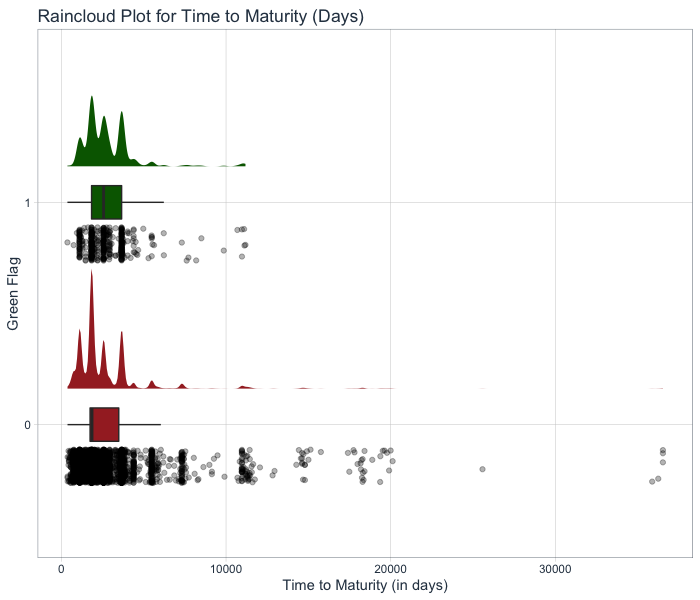
\includegraphics[scale=0.45]{chinchilab-template/chapters/appendices/ANALYSIS/rainplot4_ttm.png}
    \caption{Raincloud Plot for Time to Maturity (Days)}
    \label{fig:my_label}
\end{figure}

\begin{figure}[h!]
    \centering
    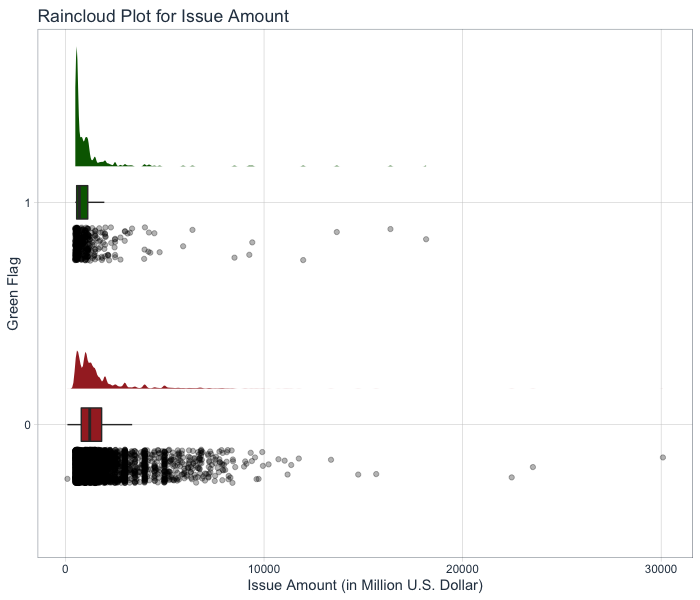
\includegraphics[scale=0.45]{chinchilab-template/chapters/appendices/ANALYSIS/rainplot4_size.png}
    \caption{Raincloud for Issue Amount}
    \label{fig:my_label}
\end{figure}

\begin{figure}[h!]
    \centering
    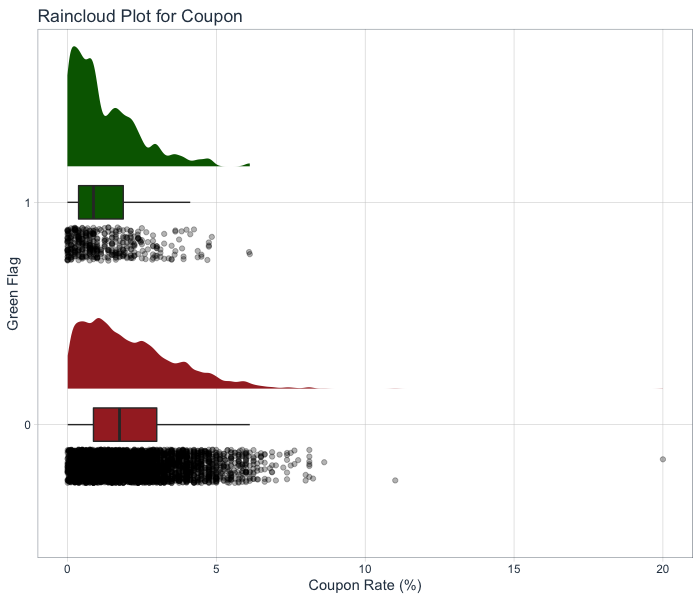
\includegraphics[scale=0.47]{chinchilab-template/chapters/appendices/ANALYSIS/rainplot4_coupon.png}
    \caption{Raincloud for Coupon Rate}
    \label{fig:my_label}
\end{figure}

\begin{figure}[h!]
    \centering
    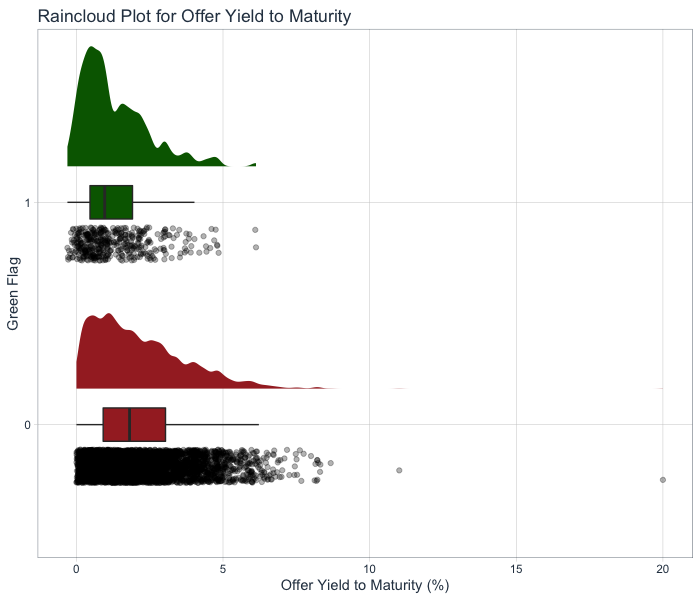
\includegraphics[scale=0.47]{chinchilab-template/chapters/appendices/ANALYSIS/rainplot4_oytm.png}
    \caption{Raincloud for Issuance Yield}
    \label{fig:my_label}
\end{figure}

\newpage

%%%%%%%%%%%%%%%%%%%%%%%%%%%%%%%%%%%%%%%%%%%%%%%%%%%%%%%%%%%%
\subsection{D.1.3 Correlation}
%%%%%%%%%%%%%%%%%%%%%%%%%%%%%%%%%%%%%%%%%%%%%%%%%%%%%%%%%%%%

\begin{figure}[h!]
    \centering
    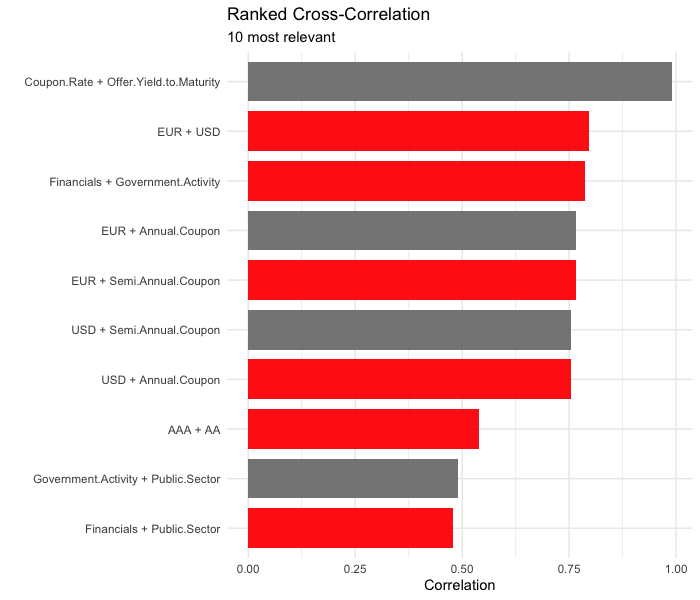
\includegraphics[scale=0.45]{chinchilab-template/chapters/appendices/ANALYSIS/correlation4.png}
    \caption{Ranked Cross-Correlation of 10 Most Relevant Pairs}
    \caption*{Note: Blue = Positive Correlation, Red = Negative Correlation.}
    \label{fig:my_label}
\end{figure}

%%%%%%%%%%%%%%%%%%%%%%%%%%%%%%%%%%%%%%%%%%%%%%%%%%%%%%%%%%%%
\subsection{D.1.4 Propensity Tables}
%%%%%%%%%%%%%%%%%%%%%%%%%%%%%%%%%%%%%%%%%%%%%%%%%%%%%%%%%%%%

\begin{table}[H]{
    \begin{subtable}{.5\textwidth}
    \footnotesize
    \centering
        {\begin{tabular}{lll}
        \\[-1.8ex]\hline 
        \hline \\[-1.8ex] 
        \textbf{Issue Year} & \textbf{Green (\%)} & \textbf{Brown (\%)} \\
        \hline \\[-1.8ex]
        {\color[HTML]{333333} 2008} & \cellcolor[HTML]{FFFFFF}{\color[HTML]{333333} 0.0} & \cellcolor[HTML]{E9F0E6}{\color[HTML]{333333} 4.8} \\
        \cellcolor[HTML]{FAFAFA}{\color[HTML]{333333} 2009} & \cellcolor[HTML]{FFFFFF}{\color[HTML]{333333} 0.0} & \cellcolor[HTML]{CEDEC8}{\color[HTML]{333333} 5.3} \\
        {\color[HTML]{333333} 2010} & \cellcolor[HTML]{FFFFFF}{\color[HTML]{333333} 0.0} & \cellcolor[HTML]{6E9C61}{\color[HTML]{333333} 7.1} \\
        \cellcolor[HTML]{FAFAFA}{\color[HTML]{333333} 2011} & \cellcolor[HTML]{FFFFFF}{\color[HTML]{333333} 0.0} & \cellcolor[HTML]{84AB77}{\color[HTML]{333333} 6.7} \\
        {\color[HTML]{333333} 2012} & \cellcolor[HTML]{FCFDFC}{\color[HTML]{333333} 0.2} & \cellcolor[HTML]{006400}{\color[HTML]{FFFFFF} 8.7} \\
        \cellcolor[HTML]{FAFAFA}{\color[HTML]{333333} 2013} & \cellcolor[HTML]{E7EFE4}{\color[HTML]{333333} 1.9} & \cellcolor[HTML]{598E4B}{\color[HTML]{FFFFFF} 7.5} \\
        {\color[HTML]{333333} 2014} & \cellcolor[HTML]{E7EFE4}{\color[HTML]{333333} 1.9} & \cellcolor[HTML]{598E4B}{\color[HTML]{FFFFFF} 7.5} \\
        \cellcolor[HTML]{FAFAFA}{\color[HTML]{333333} 2015} & \cellcolor[HTML]{BBD1B3}{\color[HTML]{333333} 5.4} & \cellcolor[HTML]{36792A}{\color[HTML]{FFFFFF} 8.1} \\
        {\color[HTML]{333333} 2016} & \cellcolor[HTML]{A4C19A}{\color[HTML]{333333} 7.3} & \cellcolor[HTML]{29721E}{\color[HTML]{FFFFFF} 8.3} \\
        \cellcolor[HTML]{FAFAFA}{\color[HTML]{333333} 2017} & \cellcolor[HTML]{88AD7C}{\color[HTML]{333333} 9.6} & \cellcolor[HTML]{69995B}{\color[HTML]{333333} 7.2} \\
        {\color[HTML]{333333} 2018} & \cellcolor[HTML]{7CA56F}{\color[HTML]{333333} 10.6} & \cellcolor[HTML]{74A066}{\color[HTML]{333333} 7.0} \\
        \cellcolor[HTML]{FAFAFA}{\color[HTML]{333333} 2019} & \cellcolor[HTML]{29721E}{\color[HTML]{FFFFFF} 16.9} & \cellcolor[HTML]{598E4B}{\color[HTML]{FFFFFF} 7.5} \\
        {\color[HTML]{333333} 2020} & \cellcolor[HTML]{6A9A5D}{\color[HTML]{333333} 12.0} & \cellcolor[HTML]{D9E5D4}{\color[HTML]{333333} 5.1} \\
        \cellcolor[HTML]{FAFAFA}{\color[HTML]{333333} 2021} & \cellcolor[HTML]{006400}{\color[HTML]{FFFFFF} 18.6} & \cellcolor[HTML]{FFFFFF}{\color[HTML]{333333} 4.4} \\
        {\color[HTML]{333333} 2022} & \cellcolor[HTML]{3D7D30}{\color[HTML]{FFFFFF} 15.5} & \cellcolor[HTML]{E4ECE0}{\color[HTML]{333333} 4.9} \\
        \hline \\[-1.8ex]
        \end{tabular}}
    \subcaption{Issue Year}
    \label{propyear}
    \end{subtable}
    \begin{subtable}{0.3\linewidth}
    \footnotesize
    \centering
        {\begin{tabular}{lll}
        \\[-1.8ex]\hline 
        \hline \\[-1.8ex] 
        \textbf{Rating} & \textbf{Green (\%)} & \textbf{Brown (\%)} \\
        \hline \\[-1.8ex]
        AAA & \cellcolor[HTML]{006400}{\color[HTML]{FFFFFF} 32.0} & \cellcolor[HTML]{006400}{\color[HTML]{FFFFFF} 47.8} \\
        \cellcolor[HTML]{FAFAFA}AA & \cellcolor[HTML]{74A067}19.3 & \cellcolor[HTML]{82A975}25.9 \\
        A & \cellcolor[HTML]{598E4B}{\color[HTML]{FFFFFF} 23.1} & \cellcolor[HTML]{BDD2B5}13.6 \\
        \cellcolor[HTML]{FAFAFA}BBB & \cellcolor[HTML]{4E8740}{\color[HTML]{FFFFFF} 24.5} & \cellcolor[HTML]{C5D8BE}11.8 \\
        BB & \cellcolor[HTML]{F6F9F5}1.2 & \cellcolor[HTML]{FCFDFB}0.7 \\
        \cellcolor[HTML]{FAFAFA}B & \cellcolor[HTML]{FFFFFF}0.0 & \cellcolor[HTML]{FFFFFE}0.1 \\
        CCC & \cellcolor[HTML]{FFFFFF}0.0 & \cellcolor[HTML]{FFFFFF}0.0 \\
        \hline \\[-1.8ex]
        \end{tabular}}
    \subcaption{Rating}
    \label{proprating}
    \end{subtable}
\caption{Propensity Tables}}
\end{table}

\begin{table}[h!]
\centering
\caption{Propensity Table for Coupon Frequency}
\footnotesize
\begin{tabular}{lll}
\\[-1.8ex]\hline 
\hline \\[-1.8ex] 
\cellcolor[HTML]{FFFFFF}{\color[HTML]{333333} \textbf{Coupon Frequency}} & {\color[HTML]{333333} \textbf{Green (\%)}} & {\color[HTML]{333333} \textbf{Brown (\%)}} \\
\hline \\[-1.8ex] 
Annual Coupon & \cellcolor[HTML]{006400}{\color[HTML]{FFFFFF} 71.6} & \cellcolor[HTML]{006400}{\color[HTML]{FFFFFF} 65.2} \\
\cellcolor[HTML]{FAFAFA}Semi Annual Coupon & \cellcolor[HTML]{A4C099}28.2 & \cellcolor[HTML]{85AB78}34.6 \\
Quarterly & \cellcolor[HTML]{FFFFFF}0.0 & 0.2 \\
\cellcolor[HTML]{FAFAFA}Maturity & \cellcolor[HTML]{FEFFFE}0.2 & 0.1 \\
\hline \\[-1.8ex] 
\end{tabular}
\end{table}

\begin{table}[h!] \centering
\caption{Propensity Table for Industry}
\footnotesize
\begin{tabular}{lll}
\\[-1.8ex]\hline 
\hline \\[-1.8ex] 
{\color[HTML]{333333} Academic \& Educational Services} & {\color[HTML]{333333} 0.0} & {\color[HTML]{333333} 0.0} \\
\cellcolor[HTML]{FAFAFA}{\color[HTML]{333333} Basic Materials} & \cellcolor[HTML]{FCFDFC}{\color[HTML]{333333} 0.7} & \cellcolor[HTML]{FFFFFF}{\color[HTML]{333333} 0.1} \\
\cellcolor[HTML]{FFFFFF}{\color[HTML]{333333} Consumer Cyclicals} & \cellcolor[HTML]{FCFDFC}{\color[HTML]{333333} 0.7} & \cellcolor[HTML]{FDFEFD}{\color[HTML]{333333} 0.5} \\
\cellcolor[HTML]{FAFAFA}{\color[HTML]{333333} Consumer Non-Cyclicals} & \cellcolor[HTML]{FCFDFC}{\color[HTML]{333333} 0.7} & \cellcolor[HTML]{FFFFFF}{\color[HTML]{333333} 0.1} \\
\rowcolor[HTML]{FFFFFF} 
{\color[HTML]{333333} Energy} & {\color[HTML]{333333} 0.0} & {\color[HTML]{333333} 0.0} \\
\rowcolor[HTML]{006400} 
\cellcolor[HTML]{FAFAFA}{\color[HTML]{333333} Financials} & {\color[HTML]{FFFFFF} 64.0} & {\color[HTML]{FFFFFF} 71.6} \\
\cellcolor[HTML]{FFFFFF}{\color[HTML]{333333} Government Activity} & \cellcolor[HTML]{C5D7BE}{\color[HTML]{333333} 16.0} & \cellcolor[HTML]{BBD1B3}{\color[HTML]{333333} 20.8} \\
\cellcolor[HTML]{FAFAFA}{\color[HTML]{333333} Healthcare} & \cellcolor[HTML]{FEFEFE}{\color[HTML]{333333} 0.2} & \cellcolor[HTML]{FFFFFF}{\color[HTML]{333333} 0.0} \\
\cellcolor[HTML]{FFFFFF}{\color[HTML]{333333} Industrials} & \cellcolor[HTML]{EEF4EC}{\color[HTML]{333333} 4.5} & \cellcolor[HTML]{FDFDFC}{\color[HTML]{333333} 0.7} \\
\cellcolor[HTML]{FAFAFA}{\color[HTML]{333333} Institutions, Associations \& Organizations} & \cellcolor[HTML]{F0F5EE}{\color[HTML]{333333} 4.0} & \cellcolor[HTML]{F0F4EE}{\color[HTML]{333333} 4.7} \\
\rowcolor[HTML]{FFFFFF} 
{\color[HTML]{333333} Real Estate} & \cellcolor[HTML]{F6F9F5}{\color[HTML]{333333} 2.4} & {\color[HTML]{333333} 0.1} \\
\cellcolor[HTML]{FAFAFA}{\color[HTML]{333333} Technology} & \cellcolor[HTML]{FBFCFA}{\color[HTML]{333333} 1.2} & \cellcolor[HTML]{FEFEFE}{\color[HTML]{333333} 0.4} \\
\cellcolor[HTML]{FFFFFF}{\color[HTML]{333333} Utilities} & \cellcolor[HTML]{EAF1E8}{\color[HTML]{333333} 5.6} & \cellcolor[HTML]{FCFDFB}{\color[HTML]{333333} 1.0} \\
\hline \\[-1.8ex] 
\end{tabular}
\end{table}

\begin{table}[h!] \centering
\caption{Propensity Table for Currency}
\footnotesize
\begin{tabular}{llllll}
\\[-1.8ex]\hline 
\hline \\[-1.8ex] 
\textbf{Currency} & \textbf{Green (\%)} & \textbf{Brown (\%)} \\
\hline \\[-1.8ex]
{\color[HTML]{333333} AUD} & \cellcolor[HTML]{FDFDFC}{\color[HTML]{333333} 0.7} & \cellcolor[HTML]{F8FAF7}{\color[HTML]{333333} 1.6} \\
\cellcolor[HTML]{FAFAFA}{\color[HTML]{333333} BRL} & {\color[HTML]{333333} 0.0} & {\color[HTML]{333333} 0.0} \\
{\color[HTML]{333333} CAD} & \cellcolor[HTML]{F6F9F5}{\color[HTML]{333333} 2.4} & \cellcolor[HTML]{FDFDFC}{\color[HTML]{333333} 0.5} \\
\cellcolor[HTML]{FAFAFA}{\color[HTML]{333333} CLP} & {\color[HTML]{333333} 0.0} & {\color[HTML]{333333} 0.0} \\
{\color[HTML]{333333} CNY} & \cellcolor[HTML]{FEFFFE}{\color[HTML]{333333} 0.2} & {\color[HTML]{333333} 0.0} \\
\cellcolor[HTML]{FAFAFA}{\color[HTML]{333333} COP} & {\color[HTML]{333333} 0.0} & {\color[HTML]{333333} 0.0} \\
{\color[HTML]{333333} HRK} & {\color[HTML]{333333} 0.0} & {\color[HTML]{333333} 0.0} \\
\cellcolor[HTML]{FAFAFA}{\color[HTML]{333333} EUR} & \cellcolor[HTML]{006400}{\color[HTML]{FFFFFF} 66.6} & \cellcolor[HTML]{006400}{\color[HTML]{FFFFFF} 52.5} \\
{\color[HTML]{333333} GBP} & \cellcolor[HTML]{F9FBF9}{\color[HTML]{333333} 1.6} & \cellcolor[HTML]{E0EADC}{\color[HTML]{333333} 6.9} \\
\cellcolor[HTML]{FAFAFA}{\color[HTML]{333333} HKD} & {\color[HTML]{333333} 0.0} & {\color[HTML]{333333} 0.0} \\
{\color[HTML]{333333} JPY} & \cellcolor[HTML]{FEFFFE}{\color[HTML]{333333} 0.2} & \cellcolor[HTML]{F7FAF6}{\color[HTML]{333333} 1.7} \\
\cellcolor[HTML]{FAFAFA}{\color[HTML]{333333} KZT} & {\color[HTML]{333333} 0.0} & {\color[HTML]{333333} 0.0} \\
{\color[HTML]{333333} MXN} & {\color[HTML]{333333} 0.0} & {\color[HTML]{333333} 0.0} \\
\cellcolor[HTML]{FAFAFA}{\color[HTML]{333333} NZD} & {\color[HTML]{333333} 0.0} & \cellcolor[HTML]{FFFFFE}{\color[HTML]{333333} 0.1} \\
{\color[HTML]{333333} NOK} & \cellcolor[HTML]{FEFFFE}{\color[HTML]{333333} 0.2} & {\color[HTML]{333333} 0.0} \\
\cellcolor[HTML]{FAFAFA}{\color[HTML]{333333} PEN} & {\color[HTML]{333333} 0.0} & {\color[HTML]{333333} 0.0} \\
{\color[HTML]{333333} PHP} & {\color[HTML]{333333} 0.0} & {\color[HTML]{333333} 0.0} \\
\cellcolor[HTML]{FAFAFA}{\color[HTML]{333333} RUB} & {\color[HTML]{333333} 0.0} & {\color[HTML]{333333} 0.0} \\
{\color[HTML]{333333} SGD} & {\color[HTML]{333333} 0.0} & {\color[HTML]{333333} 0.0} \\
\cellcolor[HTML]{FAFAFA}{\color[HTML]{333333} SEK} & \cellcolor[HTML]{FAFCF9}{\color[HTML]{333333} 1.4} & {\color[HTML]{333333} 0.0} \\
{\color[HTML]{333333} CHF} & {\color[HTML]{333333} 0.0} & \cellcolor[HTML]{FEFEFE}{\color[HTML]{333333} 0.2} \\
\cellcolor[HTML]{FAFAFA}{\color[HTML]{333333} THB} & {\color[HTML]{333333} 0.0} & {\color[HTML]{333333} 0.0} \\
{\color[HTML]{333333} TRY} & {\color[HTML]{333333} 0.0} & {\color[HTML]{333333} 0.0} \\
\cellcolor[HTML]{FAFAFA}{\color[HTML]{333333} USD} & \cellcolor[HTML]{A2C098}{\color[HTML]{333333} 26.6} & \cellcolor[HTML]{609352}{\color[HTML]{FFFFFF} 36.2} \\
{\color[HTML]{333333} UYU} & {\color[HTML]{333333} 0.0} & {\color[HTML]{333333} 0.0} \\
\hline \\[-1.8ex]
\end{tabular}
\end{table}

\begin{table}[h!] \centering
\caption{Propensity Table for Seniority}
\footnotesize
\begin{tabular}{llllll}
\\[-1.8ex]\hline 
\hline \\[-1.8ex] 
\cellcolor[HTML]{FFFFFF}{\color[HTML]{333333} \textbf{Seniority}} & \cellcolor[HTML]{FFFFFF}{\color[HTML]{333333} \textbf{Green (\%)}} & \cellcolor[HTML]{FFFFFF}{\color[HTML]{333333} \textbf{Brown (\%)}} \\
\hline \\[-1.8ex]
{\color[HTML]{333333} First-Lien Loan} & {\color[HTML]{333333} 0.0} & {\color[HTML]{333333} 0.0} \\
\cellcolor[HTML]{FAFAFA}{\color[HTML]{333333} First Mortgage} & {\color[HTML]{333333} 0.0} & {\color[HTML]{333333} 0.0} \\
{\color[HTML]{333333} First Refunding Mortgage} & {\color[HTML]{333333} 0.0} & {\color[HTML]{333333} 0.0} \\
\cellcolor[HTML]{FAFAFA}{\color[HTML]{333333} Second-Lien Loan} & {\color[HTML]{333333} 0.0} & {\color[HTML]{333333} 0.0} \\
{\color[HTML]{333333} Junior Subordinated} & {\color[HTML]{333333} 0.0} & {\color[HTML]{333333} 0.0} \\
\cellcolor[HTML]{FAFAFA}{\color[HTML]{333333} Senior Secured Mortgage} & \cellcolor[HTML]{DFE9DB}{\color[HTML]{333333} 9.2} & \cellcolor[HTML]{D9E5D4}{\color[HTML]{333333} 10.2} \\
{\color[HTML]{333333} Refunding Mortgage} & {\color[HTML]{333333} 0.0} & {\color[HTML]{333333} 0.0} \\
\cellcolor[HTML]{FAFAFA}{\color[HTML]{333333} Senior Secured} & \cellcolor[HTML]{006400}{\color[HTML]{FFFFFF} 67.3} & \cellcolor[HTML]{006400}{\color[HTML]{FFFFFF} 62.7} \\
{\color[HTML]{333333} Senior Unsecured} & \cellcolor[HTML]{E1EBDE}{\color[HTML]{333333} 8.5} & \cellcolor[HTML]{F2F6F0}{\color[HTML]{333333} 3.5} \\
\cellcolor[HTML]{FAFAFA}{\color[HTML]{333333} Senior Non-Preferred} & \cellcolor[HTML]{DCE7D8}{\color[HTML]{333333} 9.9} & \cellcolor[HTML]{EAF1E8}{\color[HTML]{333333} 5.5} \\
{\color[HTML]{333333} Senior Preferred} & \cellcolor[HTML]{F9FBF9}{\color[HTML]{333333} 1.6} & \cellcolor[HTML]{E9F0E6}{\color[HTML]{333333} 5.9} \\
\cellcolor[HTML]{FAFAFA}{\color[HTML]{333333} Senior Subordinated Unsecured} & \cellcolor[HTML]{FEFFFE}{\color[HTML]{333333} 0.2} & \cellcolor[HTML]{FEFEFE}{\color[HTML]{333333} 0.3} \\
{\color[HTML]{333333} Senior Subordinated Secured} & {\color[HTML]{333333} 0.0} & {\color[HTML]{333333} 0.0} \\
\cellcolor[HTML]{FAFAFA}{\color[HTML]{333333} Subordinated Unsecured} & \cellcolor[HTML]{FDFDFC}{\color[HTML]{333333} 0.7} & \cellcolor[HTML]{F6F9F5}{\color[HTML]{333333} 2.4} \\
{\color[HTML]{333333} Subordinated Secured} & {\color[HTML]{333333} 0.0} & {\color[HTML]{333333} 0.0} \\
\cellcolor[HTML]{FAFAFA}{\color[HTML]{333333} Unsecured} & \cellcolor[HTML]{F7F9F5}{\color[HTML]{333333} 2.4} & \cellcolor[HTML]{E1EBDE}{\color[HTML]{333333} 7.9} \\
\hline \\[-1.8ex]
\end{tabular}
\end{table}




\begin{table}[H]{
    \begin{subtable}{.5\textwidth}
    \centering
    \footnotesize
        {\begin{tabular}{lll}
        \\[-1.8ex]\hline 
        \hline \\[-1.8ex] 
        \textbf{Issuer Sector} & \textbf{Green (\%)} & \textbf{Brown (\%)} \\
        \hline \\[-1.8ex]
        \cellcolor[HTML]{FFFFFF}{\color[HTML]{333333} Public Sector} & {\color[HTML]{333333} 52.6} & {\color[HTML]{333333} 62.8} \\
        \rowcolor[HTML]{006400} 
        \cellcolor[HTML]{FFFFFF}{\color[HTML]{333333} Corporate Sector} & {\color[HTML]{FFFFFF} 47.4} & {\color[HTML]{FFFFFF} 37.2} \\
        \\[-1.8ex]\hline 
        \end{tabular}}
    \subcaption{Issuer Sector}
    \end{subtable}
    \begin{subtable}{0.3\linewidth}
    \centering
    \footnotesize
        {\begin{tabular}{lll}
        \\[-1.8ex]\hline 
        \hline \\[-1.8ex] 
        \textbf{Guarantor} & \textbf{Green (\%)} & \textbf{Brown (\%)} \\
        \hline \\[-1.8ex]
        \rowcolor[HTML]{FFFFFF} 
        {\color[HTML]{333333} Guarantor} & {\color[HTML]{333333} 16.9} & {\color[HTML]{333333} 18.5} \\
        \rowcolor[HTML]{006400} 
        \cellcolor[HTML]{FAFAFA}{\color[HTML]{333333} No Guarantor} & {\color[HTML]{FFFFFF} 83.1} & {\color[HTML]{FFFFFF} 81.5} \\
        \hline \\[-1.8ex]
        \end{tabular}}
    \subcaption{Guarantor}
    \end{subtable}
\caption{Propensity Table for Issuer Sector and Guarantor}
\label{x}}
\end{table}

%%%%%%%%%%%%%%%%%%%%%%%%%%%%%%%%%%%%%%%%%%%%%%%%%%%%%%%%%%%%
\section{D.2 Causal Forest}
%%%%%%%%%%%%%%%%%%%%%%%%%%%%%%%%%%%%%%%%%%%%%%%%%%%%%%%%%%%%


%%%%%%%%%%%%%%%%%%%%%%%%%%%%%%%%%%%%%%%%%%%%%%%%%%%%%%%%%%%%
\subsection{D.2.1 Without Issuer Controls}
%%%%%%%%%%%%%%%%%%%%%%%%%%%%%%%%%%%%%%%%%%%%%%%%%%%%%%%%%%%%

\begin{figure}[H]
    \centering
    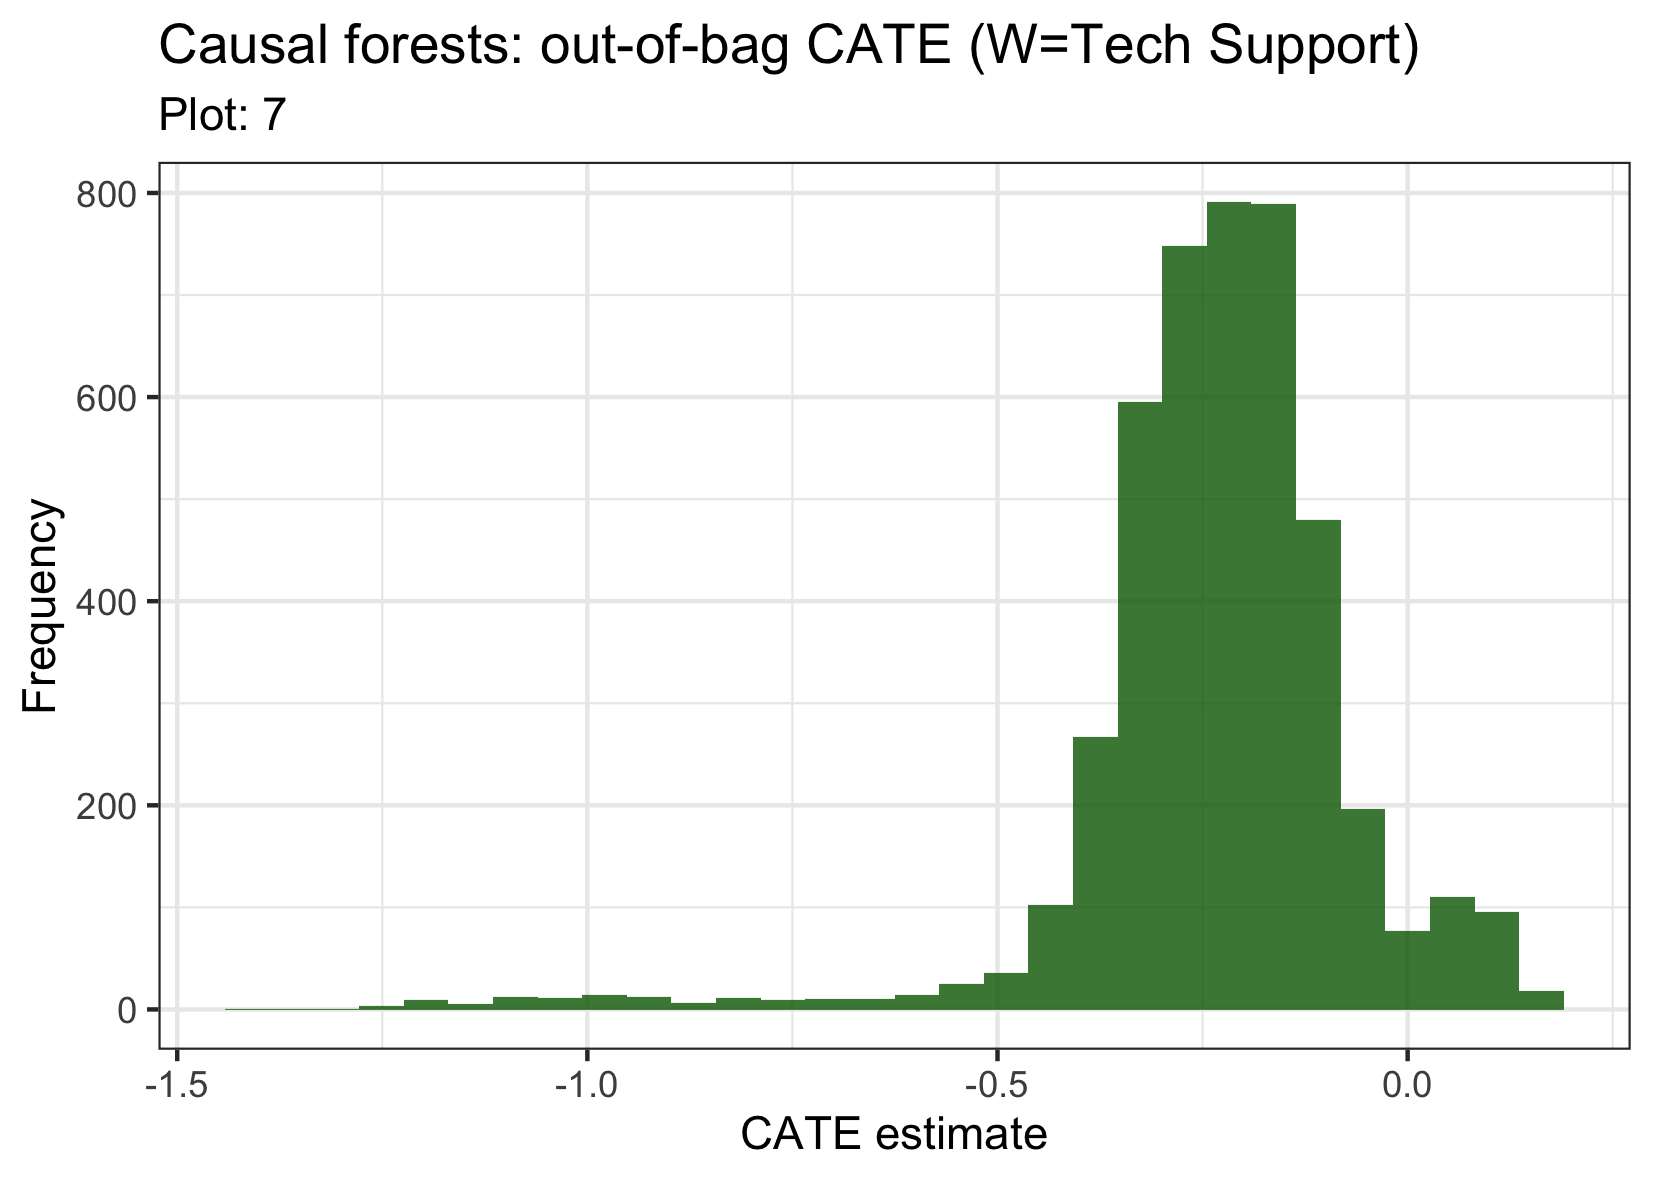
\includegraphics[scale=0.15]{chinchilab-template/chapters/appendices/ANALYSIS/CATE_7.png}
    \caption{Distribution of CATE (Model 7)}
    \label{fig:my_label}
\end{figure}

%%%%%%%%%%%%%%%%%%%%%%%%%%%%%%%%%%%%%%%%%%%%%%%%%%%%%%%%%%%%
\subsubsection{D.2.1.1 Nuisance Parameter Check}
%%%%%%%%%%%%%%%%%%%%%%%%%%%%%%%%%%%%%%%%%%%%%%%%%%%%%%%%%%%%
\begin{figure}[H]
    \centering
    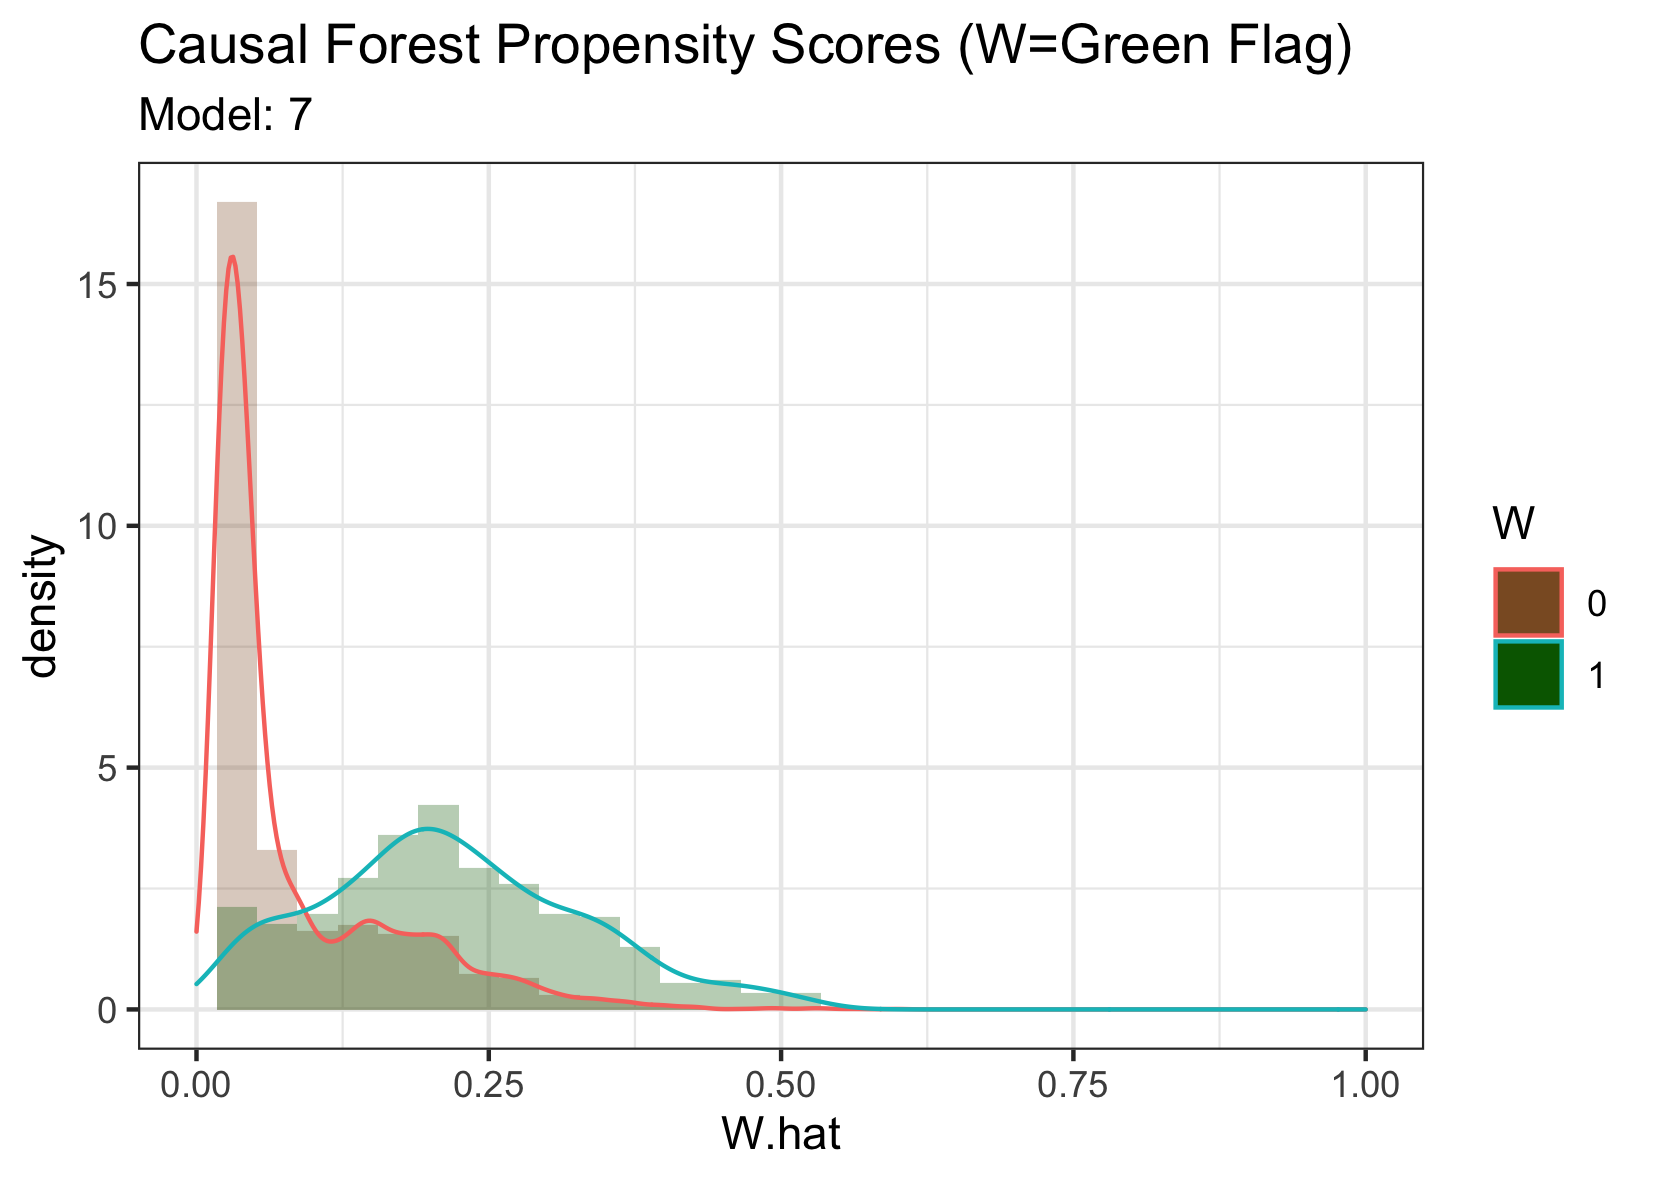
\includegraphics[scale=0.15]{chinchilab-template/chapters/appendices/ANALYSIS/prop_7.png}
    \caption{Propensity Score Distribution (Model 7)}
    \label{fig:my_label}
\end{figure}

\begin{table}[H]{
    \begin{subtable}{.5\textwidth}
    \centering
    \footnotesize
        {\begin{tabular}{@{\extracolsep{5pt}}lc} 
        \\[-1.8ex]\hline 
        \hline \\[-1.8ex] 
         & \multicolumn{1}{c}{\textit{Dependent variable: Green Flag}} \\ 
        \cline{2-2} 
        \\[-1.8ex] &   \\ 
        \hline \\[-1.8ex] 
         e.bar & 1.006$^{***}$ \\ 
          & (0.042) \\ 
          & \\ 
         e.residual & 1.323$^{***}$ \\ 
          & (0.066) \\ 
          & \\ 
        \hline \\[-1.8ex] 
        \hline 
        \hline \\[-1.8ex] 
        \textit{Note:}  & \multicolumn{1}{r}{$^{*}$p$<$0.1; $^{**}$p$<$0.05; $^{***}$p$<$0.01} \\ 
        \end{tabular}}
    \subcaption{Outcome Model}
    \end{subtable}
    \begin{subtable}{0.3\linewidth}
    \centering
    \footnotesize
        {\begin{tabular}{@{\extracolsep{5pt}}lc} 
        \\[-1.8ex]\hline 
        \hline \\[-1.8ex] 
         & \multicolumn{1}{c}{\textit{Dependent variable: Green Flag}} \\ 
        \cline{2-2} 
        \\[-1.8ex] &   \\ 
        \hline \\[-1.8ex] 
         m.bar & 0.999$^{***}$ \\ 
          & (0.013) \\ 
          & \\ 
         m.residual & 1.290$^{***}$ \\ 
          & (0.020) \\ 
          & \\ 
        \hline \\[-1.8ex] 
        \hline 
        \hline \\[-1.8ex] 
        \textit{Note:}  & \multicolumn{1}{r}{$^{*}$p$<$0.1; $^{**}$p$<$0.05; $^{***}$p$<$0.01} \\ 
        \end{tabular}}
    \subcaption{Propensity Model}
    \end{subtable}
\caption{Calibration Regressions (Model 7)}
\label{x}}
\end{table}


%%%%%%%%%%%%%%%%%%%%%%%%%%%%%%%%%%%%%%%%%%%%%%%%%%%%%%%%%%%%
\subsubsection{D.2.1.2 Heterogeneity Assessment}
%%%%%%%%%%%%%%%%%%%%%%%%%%%%%%%%%%%%%%%%%%%%%%%%%%%%%%%%%%%%
\begin{table}[h!]
\centering
\caption{Variable Importance (Model 7)}
\begin{tabular}{lr}
\\[-1.8ex]\hline 
\hline \\[-1.8ex] 
\rowcolor[HTML]{FFFFFF} 
{\color[HTML]{333333} \textbf{Covariate}} & {\color[HTML]{333333} \textbf{Value}} \\ \hline
\rowcolor[HTML]{FFFFFF} 
{\color[HTML]{333333} Issue Amount} & \cellcolor[HTML]{00441B}{\color[HTML]{FFFFFF} 0.25784685} \\
\rowcolor[HTML]{FFFFFF} 
{\color[HTML]{333333} 2022} & \cellcolor[HTML]{147C38}{\color[HTML]{FFFFFF} 0.21632832} \\
\rowcolor[HTML]{FFFFFF} 
{\color[HTML]{333333} Time to Maturity (Days)} & \cellcolor[HTML]{84CB83}{\color[HTML]{FFFFFF} 0.13669900} \\
\rowcolor[HTML]{FFFFFF} 
{\color[HTML]{333333} 2021} & \cellcolor[HTML]{E6F5E1}{\color[HTML]{333333} 0.06129829} \\
\rowcolor[HTML]{FFFFFF} 
{\color[HTML]{333333} 2017} & \cellcolor[HTML]{EEF8EA}{\color[HTML]{333333} 0.04908605} \\
\rowcolor[HTML]{FFFFFF} 
{\color[HTML]{333333} 2020} & \cellcolor[HTML]{F7FCF5}{\color[HTML]{333333} 0.03483198} \\ \hline
\end{tabular}
\end{table}

\begin{figure}[h!]
    \centering
    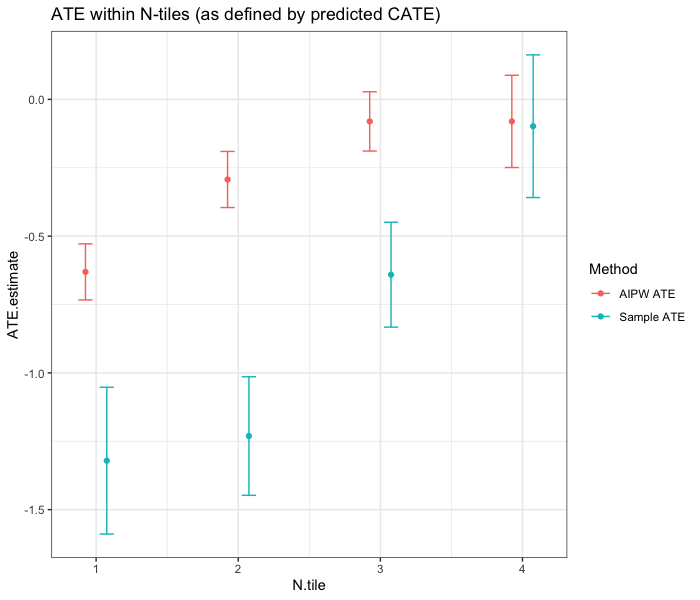
\includegraphics[scale=0.4]{chinchilab-template/chapters/appendices/ANALYSIS/ntile_cf3.png}
    \caption{Graph of ATE within Subgroups (Model 7)}
    \label{fig:my_label}
\end{figure}

\begin{figure}[H]
\centering
   \begin{subfigure}[b]{0.45\textwidth}
    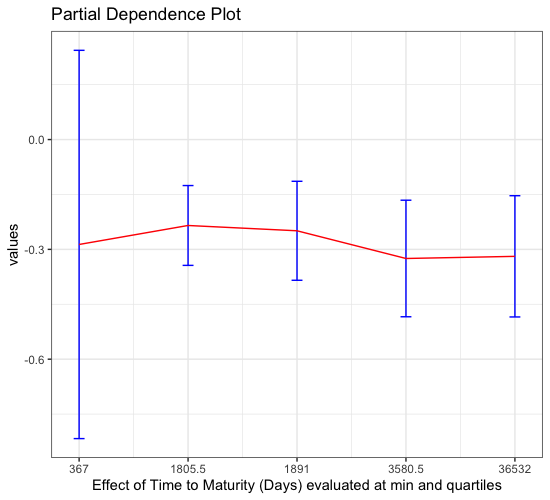
\includegraphics[width=0.8\textwidth]{chinchilab-template/chapters/appendices/ANALYSIS/PDP_cf3.png}
    \caption{Effect of Time to Maturity (Days)}
   \label{fig:Ng1} 
\end{subfigure}
\begin{subfigure}[b]{0.45\textwidth}
    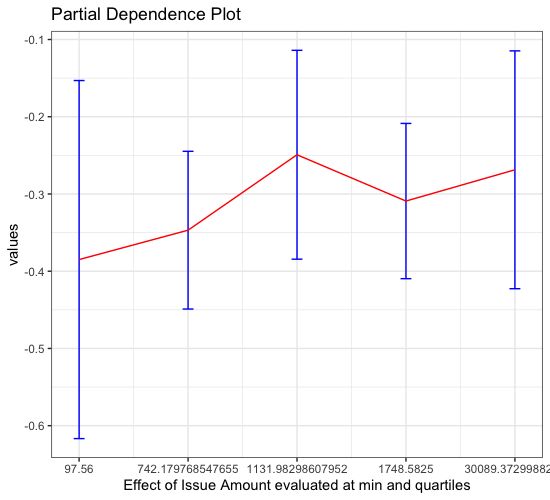
\includegraphics[width=0.8\textwidth]{chinchilab-template/chapters/appendices/ANALYSIS/PDP2_cf3.png}
    \caption{Effect of Issue Amount}
   \label{fig:Ng2}
\end{subfigure}
\\
\begin{subfigure}[b]{0.45\textwidth}
    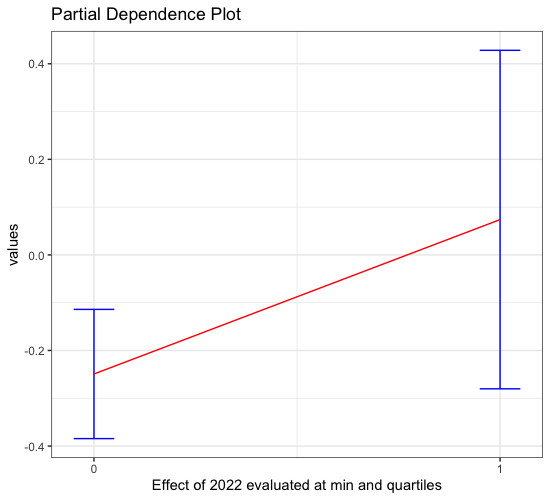
\includegraphics[width=0.8\textwidth]{chinchilab-template/chapters/appendices/ANALYSIS/PDP3_cf3.png}
    \caption{Effect of 2022}
   \label{fig:Ng2}
\end{subfigure}
\caption{Partial Dependency Plots (Model 7)}
\end{figure}

\begin{table}[H]
\caption{Heterogeneity across Covariates (Model 7)}
\label{Het}
\footnotesize
\begin{tabular}{lllll}
\\[-1.8ex]\hline 
\hline \\[-1.8ex] 
{\color[HTML]{333333} \textbf{Variable}} & {\color[HTML]{333333} \textbf{Mean ntile1}} & {\color[HTML]{333333} \textbf{Mean ntile2}} & {\color[HTML]{333333} \textbf{Mean ntile3}} & {\color[HTML]{333333} \textbf{Mean ntile4}} \\
\hline \\[-1.8ex] 
Time to   Maturity (Days) & \cellcolor[HTML]{63BE7B}3473.98 & \cellcolor[HTML]{9FD7AF}2953.37 & \cellcolor[HTML]{EDF6F3}2266.62 & \cellcolor[HTML]{FCFCFF}2135.21 \\
Issue Amount & \cellcolor[HTML]{FCFCFF}1421.98 & \cellcolor[HTML]{AEDDBC}1658.54 & \cellcolor[HTML]{C0E4CB}1604.77 & \cellcolor[HTML]{63BE7B}1885.93 \\
Guarantor & \cellcolor[HTML]{E7F4ED}0.12 & \cellcolor[HTML]{DAEFE2}0.19 & \cellcolor[HTML]{DCEFE4}0.18 & \cellcolor[HTML]{CFEAD9}0.25 \\
2013 & \cellcolor[HTML]{ECF6F2}0.09 & \cellcolor[HTML]{ECF6F2}0.09 & \cellcolor[HTML]{F2F8F6}0.06 & \cellcolor[HTML]{F5FAF9}0.04 \\
2014 & \cellcolor[HTML]{E9F4EE}0.11 & \cellcolor[HTML]{EEF7F3}0.08 & \cellcolor[HTML]{F3F9F8}0.05 & \cellcolor[HTML]{F7FAFB}0.03 \\
2015 & \cellcolor[HTML]{EAF5F0}0.1 & \cellcolor[HTML]{E9F4EE}0.11 & \cellcolor[HTML]{F0F7F5}0.07 & \cellcolor[HTML]{F5FAF9}0.04 \\
2016 & \cellcolor[HTML]{EAF5F0}0.1 & \cellcolor[HTML]{EAF5F0}0.1 & \cellcolor[HTML]{F2F8F6}0.06 & \cellcolor[HTML]{F2F8F6}0.06 \\
2017 & \cellcolor[HTML]{FCFCFF}0 & \cellcolor[HTML]{F9FBFC}0.02 & \cellcolor[HTML]{F2F8F6}0.06 & \cellcolor[HTML]{D5ECDD}0.22 \\
2018 & \cellcolor[HTML]{FBFCFE}0.01 & \cellcolor[HTML]{F3F9F8}0.05 & \cellcolor[HTML]{E7F4ED}0.12 & \cellcolor[HTML]{E9F4EE}0.11 \\
2019 & \cellcolor[HTML]{E9F4EE}0.11 & \cellcolor[HTML]{EAF5F0}0.1 & \cellcolor[HTML]{E9F4EE}0.11 & \cellcolor[HTML]{F9FBFC}0.02 \\
2020 & \cellcolor[HTML]{FBFCFE}0.01 & \cellcolor[HTML]{F5FAF9}0.04 & \cellcolor[HTML]{ECF6F2}0.09 & \cellcolor[HTML]{ECF6F2}0.09 \\
2021 & \cellcolor[HTML]{FCFCFF}0 & \cellcolor[HTML]{F2F8F6}0.06 & \cellcolor[HTML]{E1F2E8}0.15 & \cellcolor[HTML]{F9FBFC}0.02 \\
2022 & \cellcolor[HTML]{FCFCFF}0 & \cellcolor[HTML]{FCFCFF}0 & \cellcolor[HTML]{FCFCFF}0 & \cellcolor[HTML]{D1EBDA}0.24 \\
Annual Coupon & \cellcolor[HTML]{63BE7B}0.85 & \cellcolor[HTML]{74C589}0.76 & \cellcolor[HTML]{98D4A9}0.56 & \cellcolor[HTML]{B6E0C3}0.39 \\
Semi Annual   Coupon & \cellcolor[HTML]{E1F2E8}0.15 & \cellcolor[HTML]{D1EBDA}0.24 & \cellcolor[HTML]{ADDCBB}0.44 & \cellcolor[HTML]{90D1A2}0.6 \\
Quarterly & \cellcolor[HTML]{FCFCFF}0 & \cellcolor[HTML]{FCFCFF}0 & \cellcolor[HTML]{FCFCFF}0 & \cellcolor[HTML]{FCFCFF}0 \\
Senior   Secured Mortgage & \cellcolor[HTML]{E5F3EB}0.13 & \cellcolor[HTML]{E7F4ED}0.12 & \cellcolor[HTML]{EEF7F3}0.08 & \cellcolor[HTML]{EEF7F3}0.08 \\
Senior Secured & \cellcolor[HTML]{F0F7F5}0.07 & \cellcolor[HTML]{F2F8F6}0.06 & \cellcolor[HTML]{F5FAF9}0.04 & \cellcolor[HTML]{F3F9F8}0.05 \\
Senior Unsecured & \cellcolor[HTML]{86CC99}0.66 & \cellcolor[HTML]{90D1A2}0.6 & \cellcolor[HTML]{92D1A4}0.59 & \cellcolor[HTML]{82CB96}0.68 \\
Senior Non   Preferred & \cellcolor[HTML]{FCFCFF}0 & \cellcolor[HTML]{FBFCFE}0.01 & \cellcolor[HTML]{F0F7F5}0.07 & \cellcolor[HTML]{F0F7F5}0.07 \\
Senior Preferred & \cellcolor[HTML]{F9FBFC}0.02 & \cellcolor[HTML]{F7FAFB}0.03 & \cellcolor[HTML]{EAF5F0}0.1 & \cellcolor[HTML]{EEF7F3}0.08 \\
Senior   Subordinated Unsecured & \cellcolor[HTML]{FBFCFE}0.01 & \cellcolor[HTML]{FCFCFF}0 & \cellcolor[HTML]{FCFCFF}0 & \cellcolor[HTML]{FCFCFF}0 \\
Subordinated   Unsecured & \cellcolor[HTML]{F7FAFB}0.03 & \cellcolor[HTML]{F5FAF9}0.04 & \cellcolor[HTML]{FBFCFE}0.01 & \cellcolor[HTML]{FCFCFF}0 \\
Basic Materials & \cellcolor[HTML]{FCFCFF}0 & \cellcolor[HTML]{FCFCFF}0 & \cellcolor[HTML]{FCFCFF}0 & \cellcolor[HTML]{FCFCFF}0 \\
Consumer   Cyclicals & \cellcolor[HTML]{FBFCFE}0.01 & \cellcolor[HTML]{FCFCFF}0 & \cellcolor[HTML]{FCFCFF}0 & \cellcolor[HTML]{FCFCFF}0 \\
Consumer   Non Cyclicals & \cellcolor[HTML]{FCFCFF}0 & \cellcolor[HTML]{FCFCFF}0 & \cellcolor[HTML]{FCFCFF}0 & \cellcolor[HTML]{FCFCFF}0 \\
Financials & \cellcolor[HTML]{82CB96}0.68 & \cellcolor[HTML]{84CC97}0.67 & \cellcolor[HTML]{77C78D}0.74 & \cellcolor[HTML]{75C68B}0.75 \\
Healthcare & \cellcolor[HTML]{FCFCFF}0 & \cellcolor[HTML]{FCFCFF}0 & \cellcolor[HTML]{FCFCFF}0 & \cellcolor[HTML]{FCFCFF}0 \\
Industrials & \cellcolor[HTML]{F9FBFC}0.02 & \cellcolor[HTML]{FBFCFE}0.01 & \cellcolor[HTML]{FBFCFE}0.01 & \cellcolor[HTML]{FBFCFE}0.01 \\
Institutions,   Associations \& Organizations & \cellcolor[HTML]{F3F9F8}0.05 & \cellcolor[HTML]{F7FAFB}0.03 & \cellcolor[HTML]{F0F7F5}0.07 & \cellcolor[HTML]{F7FAFB}0.03 \\
Real Estate & \cellcolor[HTML]{FBFCFE}0.01 & \cellcolor[HTML]{FCFCFF}0 & \cellcolor[HTML]{FCFCFF}0 & \cellcolor[HTML]{FCFCFF}0 \\
Technology & \cellcolor[HTML]{FBFCFE}0.01 & \cellcolor[HTML]{FBFCFE}0.01 & \cellcolor[HTML]{FCFCFF}0 & \cellcolor[HTML]{FCFCFF}0 \\
Utilities & \cellcolor[HTML]{F5FAF9}0.04 & \cellcolor[HTML]{FBFCFE}0.01 & \cellcolor[HTML]{FCFCFF}0 & \cellcolor[HTML]{FCFCFF}0 \\
AAA & \cellcolor[HTML]{A4D9B3}0.49 & \cellcolor[HTML]{A6D9B5}0.48 & \cellcolor[HTML]{ABDCBA}0.45 & \cellcolor[HTML]{ADDCBB}0.44 \\
AA & \cellcolor[HTML]{D1EBDA}0.24 & \cellcolor[HTML]{D3ECDC}0.23 & \cellcolor[HTML]{D1EBDA}0.24 & \cellcolor[HTML]{C5E6CF}0.31 \\
A & \cellcolor[HTML]{E0F1E7}0.16 & \cellcolor[HTML]{E1F2E8}0.15 & \cellcolor[HTML]{E0F1E7}0.16 & \cellcolor[HTML]{E9F4EE}0.11 \\
BBB & \cellcolor[HTML]{EAF5F0}0.1 & \cellcolor[HTML]{E5F3EB}0.13 & \cellcolor[HTML]{E1F2E8}0.15 & \cellcolor[HTML]{E5F3EB}0.13 \\
BB & \cellcolor[HTML]{FBFCFE}0.01 & \cellcolor[HTML]{FBFCFE}0.01 & \cellcolor[HTML]{FBFCFE}0.01 & \cellcolor[HTML]{FBFCFE}0.01 \\
AUD & \cellcolor[HTML]{F7FAFB}0.03 & \cellcolor[HTML]{FBFCFE}0.01 & \cellcolor[HTML]{F9FBFC}0.02 & \cellcolor[HTML]{FBFCFE}0.01 \\
CAD & \cellcolor[HTML]{FCFCFF}0 & \cellcolor[HTML]{FCFCFF}0 & \cellcolor[HTML]{FBFCFE}0.01 & \cellcolor[HTML]{FBFCFE}0.01 \\
CLP & \cellcolor[HTML]{FCFCFF}0 & \cellcolor[HTML]{FCFCFF}0 & \cellcolor[HTML]{FCFCFF}0 & \cellcolor[HTML]{FCFCFF}0 \\
CNY & \cellcolor[HTML]{FCFCFF}0 & \cellcolor[HTML]{FCFCFF}0 & \cellcolor[HTML]{FCFCFF}0 & \cellcolor[HTML]{FCFCFF}0 \\
EUR & \cellcolor[HTML]{79C78E}0.73 & \cellcolor[HTML]{8BCF9E}0.63 & \cellcolor[HTML]{AADBB8}0.46 & \cellcolor[HTML]{C1E4CC}0.33 \\
GBP & \cellcolor[HTML]{EEF7F3}0.08 & \cellcolor[HTML]{ECF6F2}0.09 & \cellcolor[HTML]{F3F9F8}0.05 & \cellcolor[HTML]{F5FAF9}0.04 \\
JPY & \cellcolor[HTML]{FBFCFE}0.01 & \cellcolor[HTML]{F9FBFC}0.02 & \cellcolor[HTML]{F9FBFC}0.02 & \cellcolor[HTML]{FBFCFE}0.01 \\
NZD & \cellcolor[HTML]{FCFCFF}0 & \cellcolor[HTML]{FCFCFF}0 & \cellcolor[HTML]{FCFCFF}0 & \cellcolor[HTML]{FCFCFF}0 \\
NOK & \cellcolor[HTML]{FCFCFF}0 & \cellcolor[HTML]{FCFCFF}0 & \cellcolor[HTML]{FCFCFF}0 & \cellcolor[HTML]{FCFCFF}0 \\
SEK & \cellcolor[HTML]{FCFCFF}0 & \cellcolor[HTML]{FCFCFF}0 & \cellcolor[HTML]{FCFCFF}0 & \cellcolor[HTML]{FCFCFF}0 \\
\hline \\[-1.8ex] 
\end{tabular}
\end{table}

\newpage

%%%%%%%%%%%%%%%%%%%%%%%%%%%%%%%%%%%%%%%%%%%%%%%%%%%%%%%%%%%%
\subsection{D.2.2 With Issuer Controls}
%%%%%%%%%%%%%%%%%%%%%%%%%%%%%%%%%%%%%%%%%%%%%%%%%%%%%%%%%%%%

\begin{figure}[H]
    \centering
    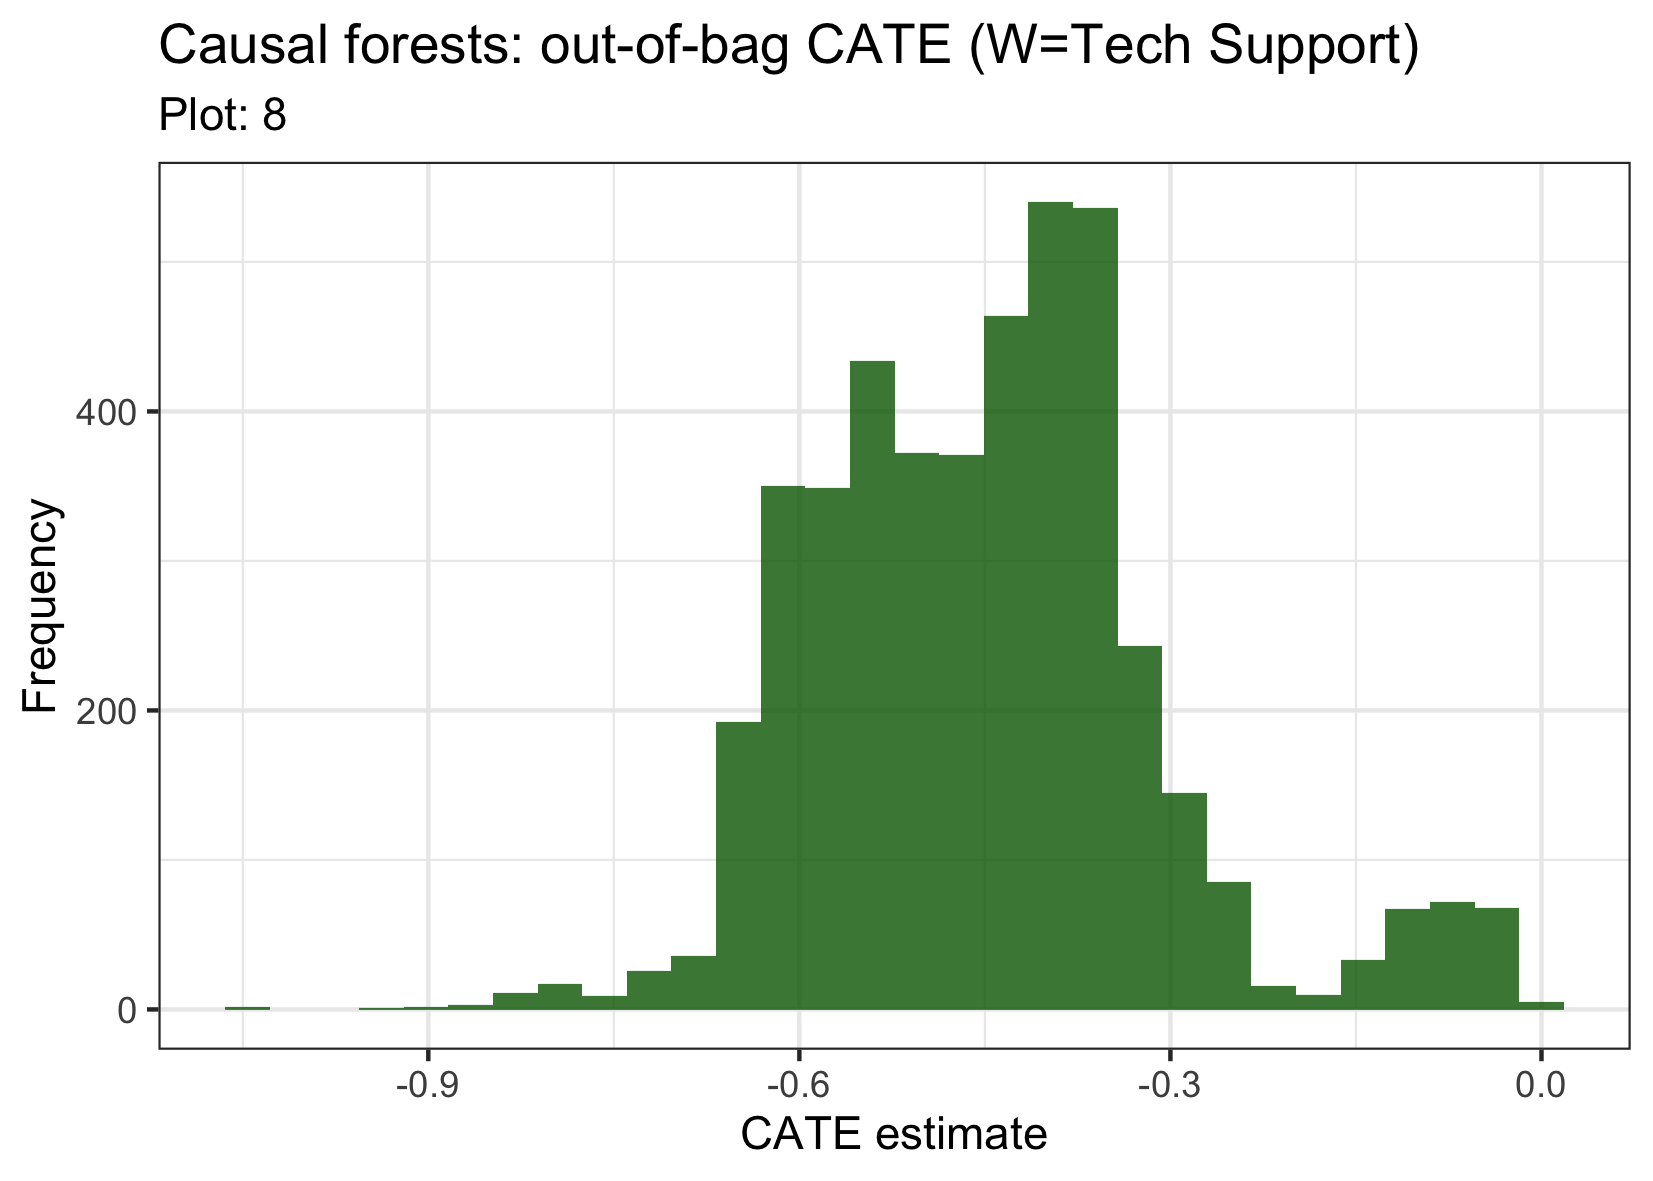
\includegraphics[scale=0.22]{chinchilab-template/chapters/appendices/ANALYSIS/CATE_8.png}
    \caption{Distribution of CATE (Model 8)}
    \label{fig:my_label}
\end{figure}

%%%%%%%%%%%%%%%%%%%%%%%%%%%%%%%%%%%%%%%%%%%%%%%%%%%%%%%%%%%%
\subsubsection{D.2.2.1 Nuisance Parameter Check}
%%%%%%%%%%%%%%%%%%%%%%%%%%%%%%%%%%%%%%%%%%%%%%%%%%%%%%%%%%%%
\begin{figure}[H]
    \centering
    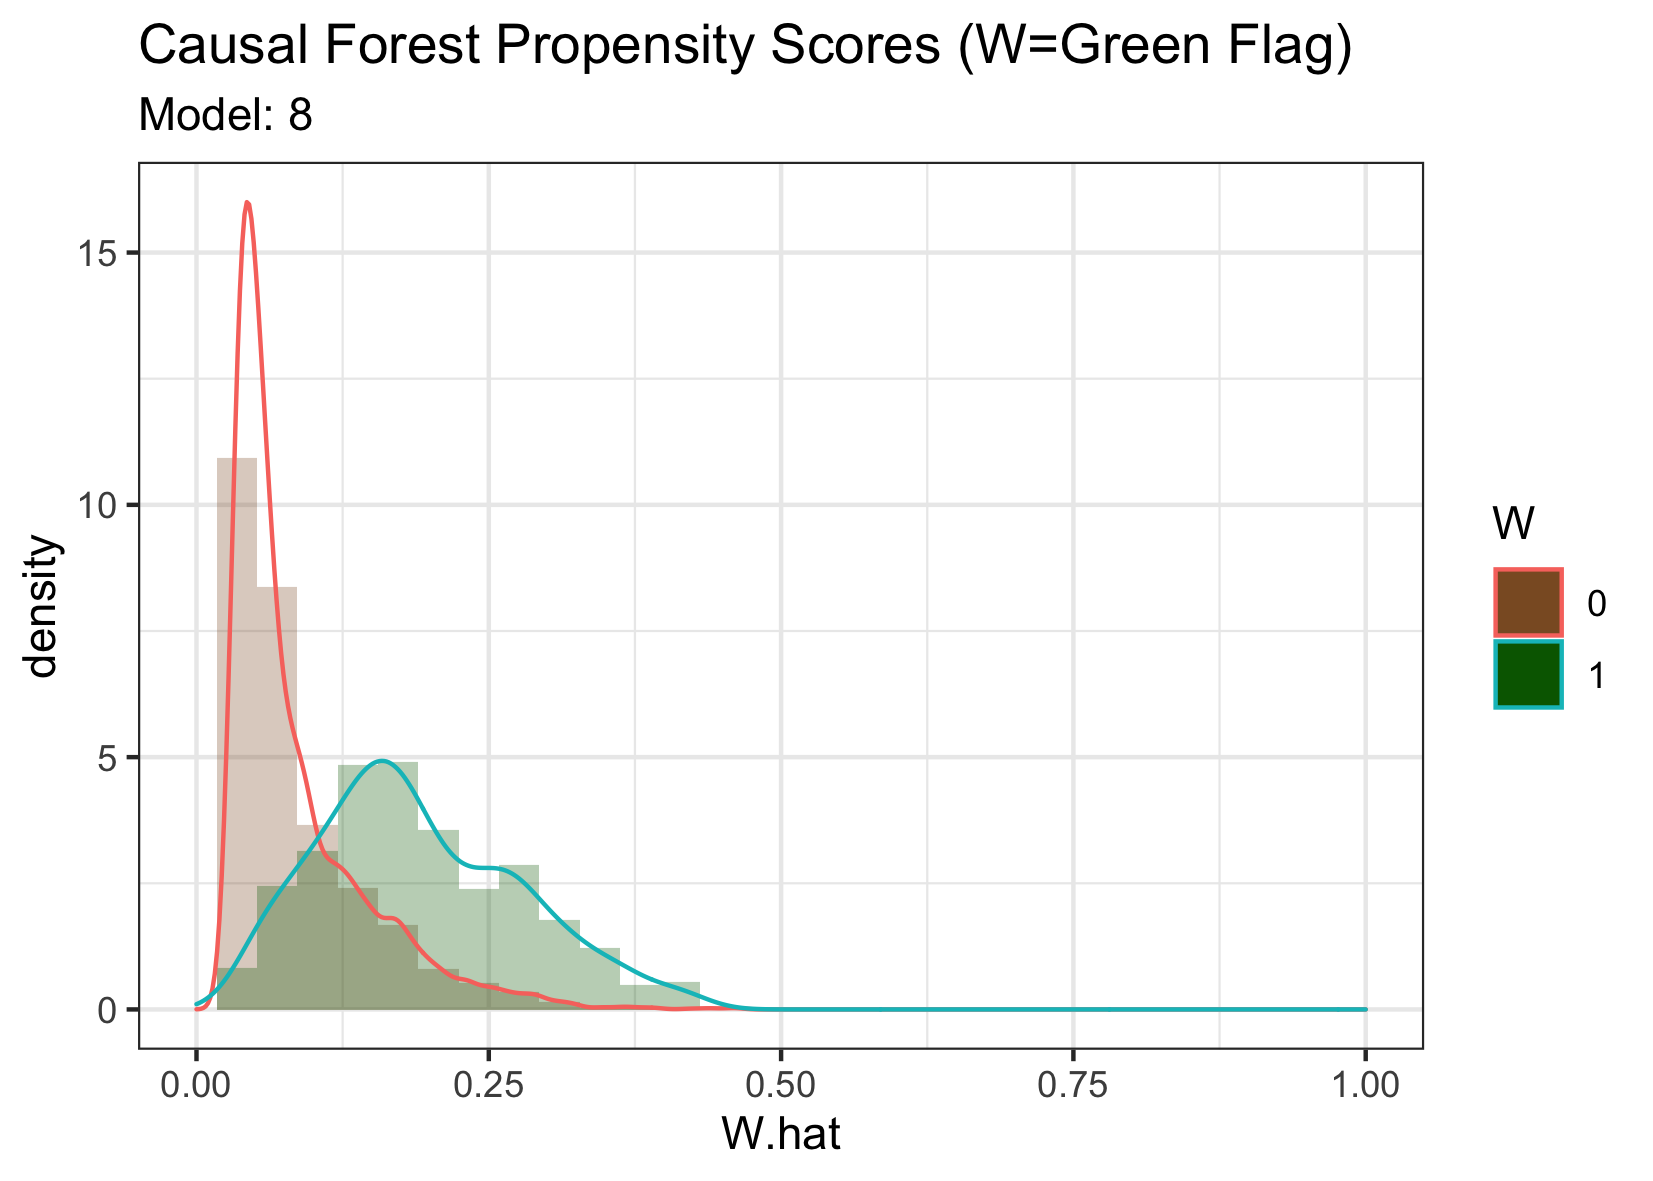
\includegraphics[scale=0.22]{chinchilab-template/chapters/appendices/ANALYSIS/prop_8.png}
    \caption{Propensity Score Distribution (Model 8)}
    \label{fig:my_label}
\end{figure}

\begin{table}[H]{
    \begin{subtable}{.5\textwidth}
    \centering
    \footnotesize
        {\begin{tabular}{@{\extracolsep{5pt}}lc} 
        \\[-1.8ex]\hline 
        \hline \\[-1.8ex] 
         & \multicolumn{1}{c}{\textit{Dependent variable: Green Flag}} \\ 
        \cline{2-2} 
        \\[-1.8ex] &   \\ 
        \hline \\[-1.8ex] 
         e.bar & 1.004$^{***}$ \\ 
          & (0.042) \\ 
          & \\ 
         e.residual & 1.863$^{***}$ \\ 
          & (0.089) \\ 
          & \\ 
        \hline \\[-1.8ex] 
        \hline 
        \hline \\[-1.8ex] 
        \textit{Note:}  & \multicolumn{1}{r}{$^{*}$p$<$0.1; $^{**}$p$<$0.05; $^{***}$p$<$0.01} \\ 
        \end{tabular} }
    \subcaption{Outcome Model}
    \end{subtable}
    \begin{subtable}{0.3\linewidth}
    \centering
    \footnotesize
        {\begin{tabular}{@{\extracolsep{5pt}}lc} 
        \\[-1.8ex]\hline 
        \hline \\[-1.8ex] 
         & \multicolumn{1}{c}{\textit{Dependent variable: Green Flag}} \\ 
        \cline{2-2} 
        \\[-1.8ex] &   \\ 
        \hline \\[-1.8ex] 
         m.bar & 1.000$^{***}$ \\ 
          & (0.013) \\ 
          & \\ 
         m.residual & 1.863$^{***}$ \\ 
          & (0.030) \\ 
          & \\ 
        \hline \\[-1.8ex] 
        \hline 
        \hline \\[-1.8ex] 
        \textit{Note:}  & \multicolumn{1}{r}{$^{*}$p$<$0.1; $^{**}$p$<$0.05; $^{***}$p$<$0.01} \\ 
        \end{tabular}}
    \subcaption{Propensity Model}
    \end{subtable}
\caption{Calibration Regressions (Model 8)}
\label{x}}
\end{table}


%%%%%%%%%%%%%%%%%%%%%%%%%%%%%%%%%%%%%%%%%%%%%%%%%%%%%%%%%%%%
\subsubsection{D.2.2.2 Heterogeneity Assessment}
%%%%%%%%%%%%%%%%%%%%%%%%%%%%%%%%%%%%%%%%%%%%%%%%%%%%%%%%%%%%
\begin{table}[h!]
\centering
\caption{Variable Importance (Model 8)}
\begin{tabular}{lr}
\\[-1.8ex]\hline 
\hline \\[-1.8ex] 
\rowcolor[HTML]{FFFFFF} 
{\color[HTML]{333333} \textbf{Covariate}} & {\color[HTML]{333333} \textbf{Value}} \\ \hline
\rowcolor[HTML]{FFFFFF} 
{\color[HTML]{333333} Issue Amount} & \cellcolor[HTML]{00441B}{\color[HTML]{FFFFFF} 0.11442882} \\
\rowcolor[HTML]{FFFFFF} 
{\color[HTML]{333333} 2022} & \cellcolor[HTML]{006729}{\color[HTML]{FFFFFF} 0.10675800} \\
\rowcolor[HTML]{FFFFFF} 
{\color[HTML]{333333} Time to Maturity (Days)} & \cellcolor[HTML]{067130}{\color[HTML]{FFFFFF} 0.10417361} \\
\rowcolor[HTML]{FFFFFF} 
{\color[HTML]{333333} 2017} & \cellcolor[HTML]{DCF1D6}{\color[HTML]{333333} 0.05447359} \\
\rowcolor[HTML]{FFFFFF} 
{\color[HTML]{333333} 2018} & \cellcolor[HTML]{EBF8E8}{\color[HTML]{333333} 0.04843323} \\
\rowcolor[HTML]{FFFFFF} 
{\color[HTML]{333333} Senior Preferred} & \cellcolor[HTML]{F7FCF5}{\color[HTML]{333333} 0.04269503} \\ \hline
\end{tabular}
\end{table}

\begin{figure}[h!]
    \centering
    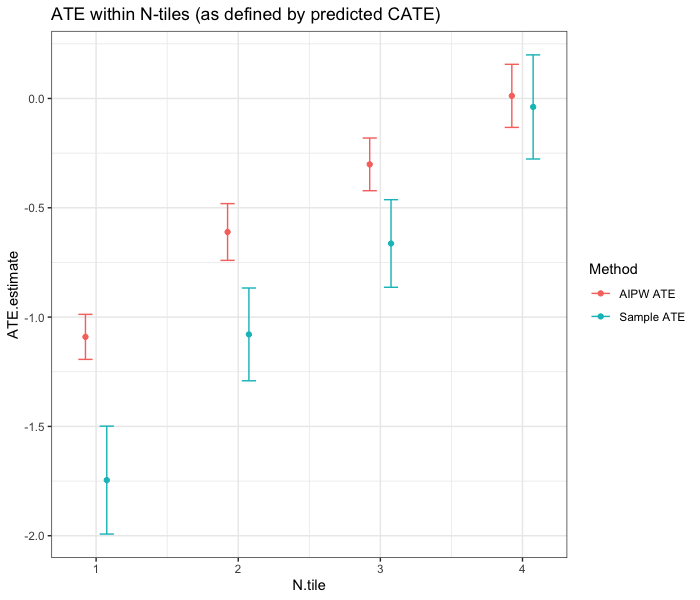
\includegraphics[scale=0.4]{chinchilab-template/chapters/appendices/ANALYSIS/ntile_3.1.png}
    \caption{Graph of ATE within Subgroups (Model 8)}
    \label{fig:my_label}
\end{figure}

\begin{figure}[H]
\centering
   \begin{subfigure}[b]{0.45\textwidth}
    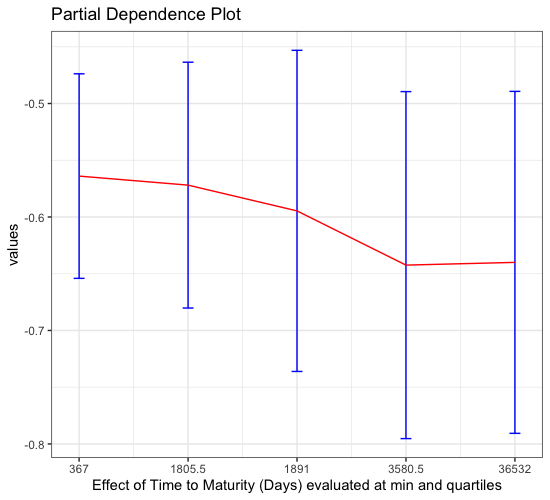
\includegraphics[width=0.9\textwidth]{chinchilab-template/chapters/appendices/ANALYSIS/PDP_cf3.1.png}
    \caption{Effect of Time to Maturity (Days)}
   \label{fig:Ng1} 
\end{subfigure}
\begin{subfigure}[b]{0.45\textwidth}
    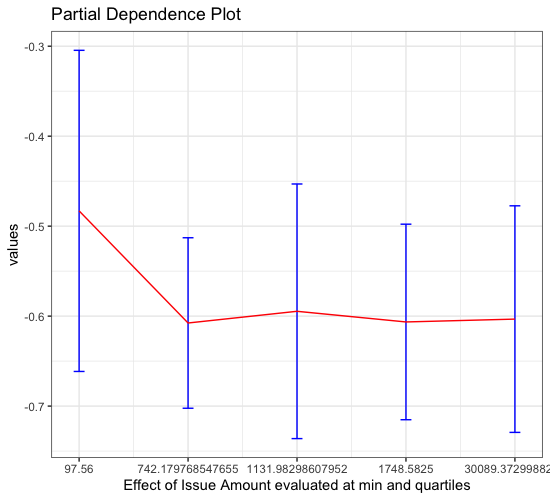
\includegraphics[width=0.9\textwidth]{chinchilab-template/chapters/appendices/ANALYSIS/PDP2_cf3.1.png}
    \caption{Effect of Issue Amount}
   \label{fig:Ng2}
\end{subfigure}
\\
\begin{subfigure}[b]{0.45\textwidth}
    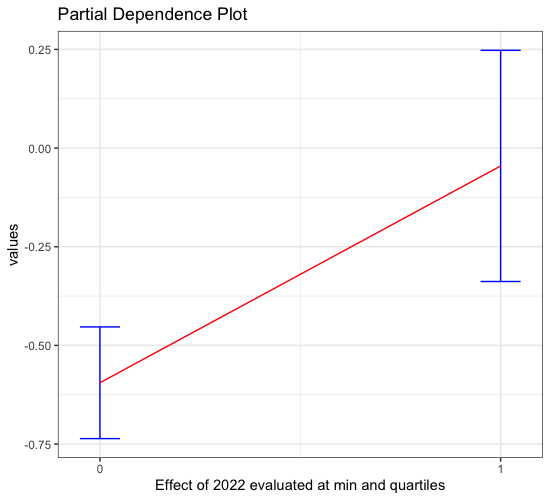
\includegraphics[width=0.9\textwidth]{chinchilab-template/chapters/appendices/ANALYSIS/PDP3_cf3.1.png}
    \caption{Effect of 2022}
   \label{fig:Ng2}
\end{subfigure}
\caption{Partial Dependency Plots (Model 8)}
\end{figure}

\begin{table}[H]
\caption{Heterogeneity across Covariates (Model 8)}
\label{Het}
\footnotesize
\begin{tabular}{lllll}
\\[-1.8ex]\hline 
\hline \\[-1.8ex] 
{\color[HTML]{333333} \textbf{Variable}} & {\color[HTML]{333333} \textbf{Mean ntile1}} & {\color[HTML]{333333} \textbf{Mean ntile2}} & {\color[HTML]{333333} \textbf{Mean ntile3}} & {\color[HTML]{333333} \textbf{Mean ntile4}} \\
\hline \\[-1.8ex] 
Time to   Maturity (Days) & \cellcolor[HTML]{63BE7B}3303.11 & \cellcolor[HTML]{6CC283}3224.23 & \cellcolor[HTML]{CFEAD8}2350.64 & \cellcolor[HTML]{FCFCFF}1951.02 \\
Issue Amount & \cellcolor[HTML]{63BE7B}1768.42 & \cellcolor[HTML]{F5F9F9}1566.89 & \cellcolor[HTML]{A4D9B3}1679.22 & \cellcolor[HTML]{FCFCFF}1556.38 \\
Guarantor & \cellcolor[HTML]{E5F3EB}0.15 & \cellcolor[HTML]{DEF0E5}0.2 & \cellcolor[HTML]{E1F1E7}0.18 & \cellcolor[HTML]{DEF0E5}0.2 \\
2013 & \cellcolor[HTML]{EAF5EF}0.12 & \cellcolor[HTML]{F3F9F7}0.06 & \cellcolor[HTML]{F0F7F5}0.08 & \cellcolor[HTML]{F9FBFD}0.02 \\
2014 & \cellcolor[HTML]{EBF6F1}0.11 & \cellcolor[HTML]{F0F7F5}0.08 & \cellcolor[HTML]{F3F9F7}0.06 & \cellcolor[HTML]{F9FBFD}0.02 \\
2015 & \cellcolor[HTML]{F3F9F7}0.06 & \cellcolor[HTML]{EBF6F1}0.11 & \cellcolor[HTML]{F0F7F5}0.08 & \cellcolor[HTML]{F3F9F7}0.06 \\
2016 & \cellcolor[HTML]{EFF7F3}0.09 & \cellcolor[HTML]{EDF6F2}0.1 & \cellcolor[HTML]{F2F8F6}0.07 & \cellcolor[HTML]{F0F7F5}0.08 \\
2017 & \cellcolor[HTML]{FCFCFF}0 & \cellcolor[HTML]{FBFCFE}0.01 & \cellcolor[HTML]{EDF6F2}0.1 & \cellcolor[HTML]{DFF1E6}0.19 \\
2018 & \cellcolor[HTML]{FCFCFF}0 & \cellcolor[HTML]{F6FAFA}0.04 & \cellcolor[HTML]{EFF7F3}0.09 & \cellcolor[HTML]{E4F2EA}0.16 \\
2019 & \cellcolor[HTML]{F6FAFA}0.04 & \cellcolor[HTML]{E5F3EB}0.15 & \cellcolor[HTML]{EDF6F2}0.1 & \cellcolor[HTML]{F5F9F9}0.05 \\
2020 & \cellcolor[HTML]{FBFCFE}0.01 & \cellcolor[HTML]{F2F8F6}0.07 & \cellcolor[HTML]{F2F8F6}0.07 & \cellcolor[HTML]{F0F7F5}0.08 \\
2021 & \cellcolor[HTML]{FBFCFE}0.01 & \cellcolor[HTML]{EFF7F3}0.09 & \cellcolor[HTML]{EDF6F2}0.1 & \cellcolor[HTML]{F9FBFD}0.02 \\
2022 & \cellcolor[HTML]{FCFCFF}0 & \cellcolor[HTML]{FCFCFF}0 & \cellcolor[HTML]{FCFCFF}0 & \cellcolor[HTML]{D7EDDF}0.24 \\
Annual Coupon & \cellcolor[HTML]{63BE7B}0.99 & \cellcolor[HTML]{84CC97}0.78 & \cellcolor[HTML]{C2E5CD}0.38 & \cellcolor[HTML]{BDE3C9}0.41 \\
Semi Annual   Coupon & \cellcolor[HTML]{FBFCFE}0.01 & \cellcolor[HTML]{DCEFE3}0.21 & \cellcolor[HTML]{9DD6AD}0.62 & \cellcolor[HTML]{A1D8B1}0.59 \\
Quarterly & \cellcolor[HTML]{FCFCFF}0 & \cellcolor[HTML]{FCFCFF}0 & \cellcolor[HTML]{FCFCFF}0 & \cellcolor[HTML]{FCFCFF}0 \\
Senior   Secured Mortgage & \cellcolor[HTML]{F9FBFD}0.02 & \cellcolor[HTML]{DFF1E6}0.19 & \cellcolor[HTML]{F2F8F6}0.07 & \cellcolor[HTML]{EBF6F1}0.11 \\
Senior Secured & \cellcolor[HTML]{F5F9F9}0.05 & \cellcolor[HTML]{F2F8F6}0.07 & \cellcolor[HTML]{F5F9F9}0.05 & \cellcolor[HTML]{F6FAFA}0.04 \\
Senior Unsecured & \cellcolor[HTML]{7EC992}0.82 & \cellcolor[HTML]{ACDCBA}0.52 & \cellcolor[HTML]{9BD5AB}0.63 & \cellcolor[HTML]{A6D9B5}0.56 \\
Senior Non   Preferred & \cellcolor[HTML]{FCFCFF}0 & \cellcolor[HTML]{FCFCFF}0 & \cellcolor[HTML]{F6FAFA}0.04 & \cellcolor[HTML]{EBF6F1}0.11 \\
Senior Preferred & \cellcolor[HTML]{FCFCFF}0 & \cellcolor[HTML]{F8FBFB}0.03 & \cellcolor[HTML]{F0F7F5}0.08 & \cellcolor[HTML]{E8F4EE}0.13 \\
Senior   Subordinated Unsecured & \cellcolor[HTML]{FBFCFE}0.01 & \cellcolor[HTML]{FCFCFF}0 & \cellcolor[HTML]{FCFCFF}0 & \cellcolor[HTML]{FCFCFF}0 \\
Subordinated   Unsecured & \cellcolor[HTML]{F9FBFD}0.02 & \cellcolor[HTML]{F6FAFA}0.04 & \cellcolor[HTML]{F9FBFD}0.02 & \cellcolor[HTML]{FCFCFF}0 \\
Basic Materials & \cellcolor[HTML]{FCFCFF}0 & \cellcolor[HTML]{FCFCFF}0 & \cellcolor[HTML]{FCFCFF}0 & \cellcolor[HTML]{FCFCFF}0 \\
Consumer   Cyclicals & \cellcolor[HTML]{F9FBFD}0.02 & \cellcolor[HTML]{FCFCFF}0 & \cellcolor[HTML]{FCFCFF}0 & \cellcolor[HTML]{FCFCFF}0 \\
Consumer   Non Cyclicals & \cellcolor[HTML]{FCFCFF}0 & \cellcolor[HTML]{FBFCFE}0.01 & \cellcolor[HTML]{FCFCFF}0 & \cellcolor[HTML]{FCFCFF}0 \\
Financials & \cellcolor[HTML]{98D4A9}0.65 & \cellcolor[HTML]{98D4A9}0.65 & \cellcolor[HTML]{8ACE9D}0.74 & \cellcolor[HTML]{82CB96}0.79 \\
Healthcare & \cellcolor[HTML]{FCFCFF}0 & \cellcolor[HTML]{FCFCFF}0 & \cellcolor[HTML]{FCFCFF}0 & \cellcolor[HTML]{FCFCFF}0 \\
Industrials & \cellcolor[HTML]{F9FBFD}0.02 & \cellcolor[HTML]{FBFCFE}0.01 & \cellcolor[HTML]{FBFCFE}0.01 & \cellcolor[HTML]{FBFCFE}0.01 \\
Institutions,   Associations \& Organizations & \cellcolor[HTML]{F6FAFA}0.04 & \cellcolor[HTML]{F8FBFB}0.03 & \cellcolor[HTML]{F0F7F5}0.08 & \cellcolor[HTML]{F6FAFA}0.04 \\
Real Estate & \cellcolor[HTML]{FCFCFF}0 & \cellcolor[HTML]{FBFCFE}0.01 & \cellcolor[HTML]{FCFCFF}0 & \cellcolor[HTML]{FCFCFF}0 \\
Technology & \cellcolor[HTML]{FBFCFE}0.01 & \cellcolor[HTML]{FBFCFE}0.01 & \cellcolor[HTML]{FCFCFF}0 & \cellcolor[HTML]{FCFCFF}0 \\
Utilities & \cellcolor[HTML]{F6FAFA}0.04 & \cellcolor[HTML]{FBFCFE}0.01 & \cellcolor[HTML]{FCFCFF}0 & \cellcolor[HTML]{FCFCFF}0 \\
AAA & \cellcolor[HTML]{BCE2C7}0.42 & \cellcolor[HTML]{AEDDBB}0.51 & \cellcolor[HTML]{AFDDBD}0.5 & \cellcolor[HTML]{BCE2C7}0.42 \\
AA & \cellcolor[HTML]{D6EDDE}0.25 & \cellcolor[HTML]{D9EEE1}0.23 & \cellcolor[HTML]{DAEFE2}0.22 & \cellcolor[HTML]{CDE9D6}0.31 \\
A & \cellcolor[HTML]{E1F1E7}0.18 & \cellcolor[HTML]{EAF5EF}0.12 & \cellcolor[HTML]{E4F2EA}0.16 & \cellcolor[HTML]{EAF5EF}0.12 \\
BBB & \cellcolor[HTML]{E8F4EE}0.13 & \cellcolor[HTML]{E7F4ED}0.14 & \cellcolor[HTML]{EAF5EF}0.12 & \cellcolor[HTML]{E7F4ED}0.14 \\
BB & \cellcolor[HTML]{FBFCFE}0.01 & \cellcolor[HTML]{FBFCFE}0.01 & \cellcolor[HTML]{FCFCFF}0 & \cellcolor[HTML]{FBFCFE}0.01 \\
AUD & \cellcolor[HTML]{FBFCFE}0.01 & \cellcolor[HTML]{F9FBFD}0.02 & \cellcolor[HTML]{F8FBFB}0.03 & \cellcolor[HTML]{FBFCFE}0.01 \\
CAD & \cellcolor[HTML]{FCFCFF}0 & \cellcolor[HTML]{FCFCFF}0 & \cellcolor[HTML]{FBFCFE}0.01 & \cellcolor[HTML]{FBFCFE}0.01 \\
CLP & \cellcolor[HTML]{FCFCFF}0 & \cellcolor[HTML]{FCFCFF}0 & \cellcolor[HTML]{FCFCFF}0 & \cellcolor[HTML]{FCFCFF}0 \\
CNY & \cellcolor[HTML]{FCFCFF}0 & \cellcolor[HTML]{FCFCFF}0 & \cellcolor[HTML]{FCFCFF}0 & \cellcolor[HTML]{FCFCFF}0 \\
EUR & \cellcolor[HTML]{78C78D}0.86 & \cellcolor[HTML]{9ED6AE}0.61 & \cellcolor[HTML]{CBE8D5}0.32 & \cellcolor[HTML]{C5E6CF}0.36 \\
GBP & \cellcolor[HTML]{F3F9F7}0.06 & \cellcolor[HTML]{EBF6F1}0.11 & \cellcolor[HTML]{F6FAFA}0.04 & \cellcolor[HTML]{F6FAFA}0.04 \\
JPY & \cellcolor[HTML]{FCFCFF}0 & \cellcolor[HTML]{FBFCFE}0.01 & \cellcolor[HTML]{F8FBFB}0.03 & \cellcolor[HTML]{F9FBFD}0.02 \\
NZD & \cellcolor[HTML]{FCFCFF}0 & \cellcolor[HTML]{FCFCFF}0 & \cellcolor[HTML]{FCFCFF}0 & \cellcolor[HTML]{FCFCFF}0 \\
NOK & \cellcolor[HTML]{FCFCFF}0 & \cellcolor[HTML]{FCFCFF}0 & \cellcolor[HTML]{FCFCFF}0 & \cellcolor[HTML]{FCFCFF}0 \\
SEK & \cellcolor[HTML]{FCFCFF}0 & \cellcolor[HTML]{FCFCFF}0 & \cellcolor[HTML]{FCFCFF}0 & \cellcolor[HTML]{FCFCFF}0 \\
\hline \\[-1.8ex] 
\end{tabular}
\end{table}


\newpage

%%%%%%%%%%%%%%%%%%%%%%%%%%%%%%%%%%%%%%%%%%%%%%%%%%%%%%%%%%%%
\subsection{D.2.3 PSM Sample}
%%%%%%%%%%%%%%%%%%%%%%%%%%%%%%%%%%%%%%%%%%%%%%%%%%%%%%%%%%%%

\begin{figure}[H]
    \centering
    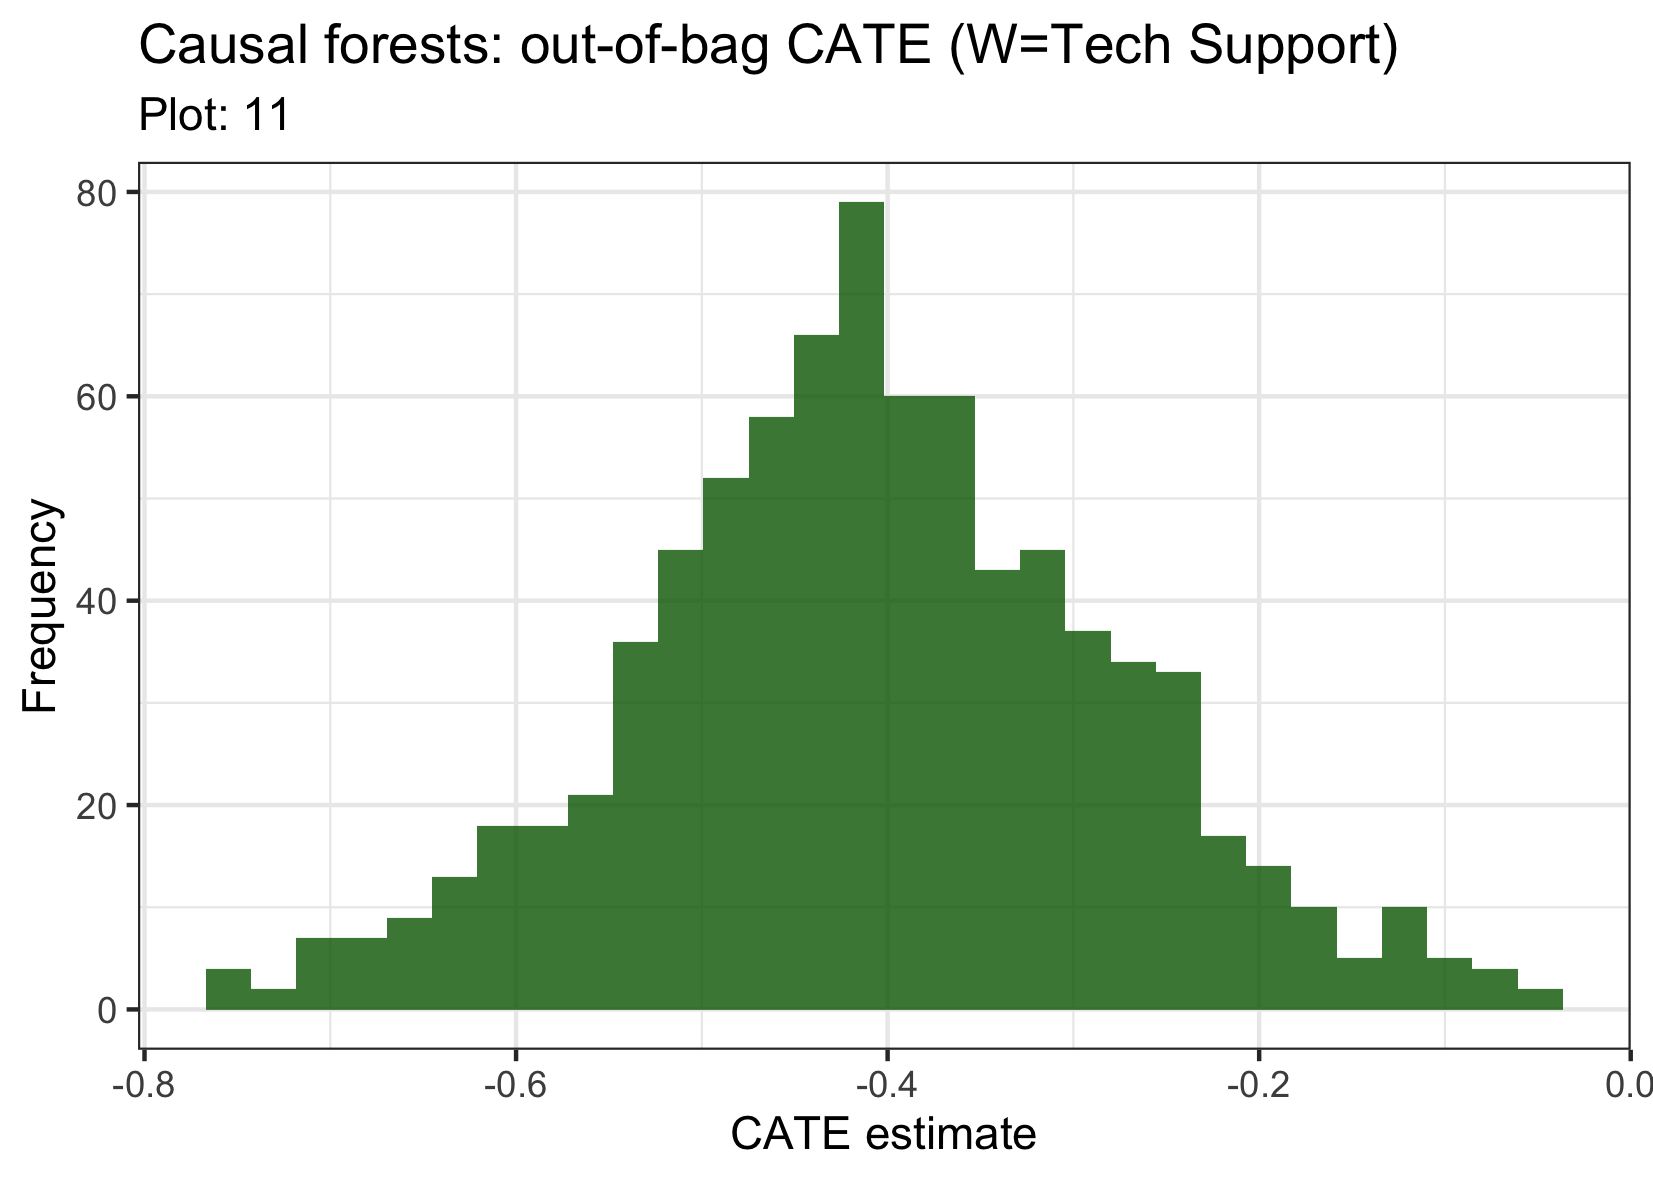
\includegraphics[scale=0.15]{chinchilab-template/chapters/appendices/ANALYSIS/CATE_11.png}
    \caption{Distribution of CATE (Model 11)}
    \label{fig:my_label}
\end{figure}

%%%%%%%%%%%%%%%%%%%%%%%%%%%%%%%%%%%%%%%%%%%%%%%%%%%%%%%%%%%%
\subsubsection{D.2.3.1 Matching Quality}
%%%%%%%%%%%%%%%%%%%%%%%%%%%%%%%%%%%%%%%%%%%%%%%%%%%%%%%%%%%%

\begin{table}[h!]
\centering
\scriptsize
\caption{Balance Check for CBI subset}
\begin{tabular}{lllll}
\\[-1.8ex]\hline 
\hline \\[-1.8ex] 
 & Std. Mean Diff. (Pre) & Std. Mean Diff. (Post) & eCDF Max (Pre) & eCDF Max (Post) \\
 \hline \\[-1.8ex] 
distance & 0.5256 & 0.3648 & 0.3347 & 0.1474 \\
MTG & -0.0359 & -0.0417 & 0.0104 & 0.0123 \\
SEC & -0.3045 & -0.1985 & 0.0148 & 0.0098 \\
SR & 0.0981 & 0.0155 & 0.0460 & 0.0074 \\
SRBN & 0.1796 & 0.1298 & 0.0500 & 0.0369 \\
SRP & 0.1484 & 0.0646 & 0.0443 & 0.0197 \\
SRSEC & -0.3341 & -0.0945 & 0.0425 & 0.0123 \\
SRSUB & -0.0128 & 0.0000 & 0.0006 & 0.0000 \\
SUB & -0.1970 & 0.0287 & 0.0165 & 0.0025 \\
UN & -0.3665 & -0.2063 & 0.0555 & 0.0319 \\
Time to Maturity (Days) & 0.0523 & 0.0135 & 0.1602 & 0.0811 \\
Guarantor & -0.0420 & 0.0386 & 0.0158 & 0.0147 \\
Australian Dollar & -0.1111 & 0.0000 & 0.0093 & 0.0000 \\
Canadian Dollar & 0.1193 & 0.0635 & 0.0181 & 0.0098 \\
Chilian Peso & -0.0234 & -0.0701 & 0.0005 & 0.0025 \\
Chinese Yuan Renminbi & 0.0434 & 0.0496 & 0.0021 & 0.0025 \\
Euro & 0.2991 & -0.0208 & 0.1411 & 0.0098 \\
Great Britain Pound & -0.4140 & -0.0189 & 0.0527 & 0.0025 \\
Japanese Yen & -0.3045 & -0.0496 & 0.0148 & 0.0025 \\
Mexican Peso & -0.0166 & -0.0701 & 0.0002 & 0.0025 \\
Norwegian Krone & 0.0383 & 0.0000 & 0.0019 & 0.0000 \\
Swedish Krona & 0.1176 & 0.1019 & 0.0139 & 0.0123 \\
Swiss Franc & -0.0469 & -0.0701 & 0.0020 & 0.0025 \\
U.S. Dollar & -0.2174 & -0.0055 & 0.0960 & 0.0025 \\
A & 0.2243 & 0.0354 & 0.0945 & 0.0147 \\
AA & -0.1675 & -0.0309 & 0.0661 & 0.0123 \\
AAA & -0.3391 & -0.0781 & 0.1582 & 0.0369 \\
BB & 0.0401 & 0.0000 & 0.0043 & 0.0000 \\
BBB & 0.2947 & 0.0810 & 0.1267 & 0.0344 \\
\hline \\[-1.8ex] 
\end{tabular}
\end{table}

\newpage

%%%%%%%%%%%%%%%%%%%%%%%%%%%%%%%%%%%%%%%%%%%%%%%%%%%%%%%%%%%%
\subsubsection{D.2.3.1 Nuisance Parameter Check}
%%%%%%%%%%%%%%%%%%%%%%%%%%%%%%%%%%%%%%%%%%%%%%%%%%%%%%%%%%%%

\begin{figure}
    \centering
    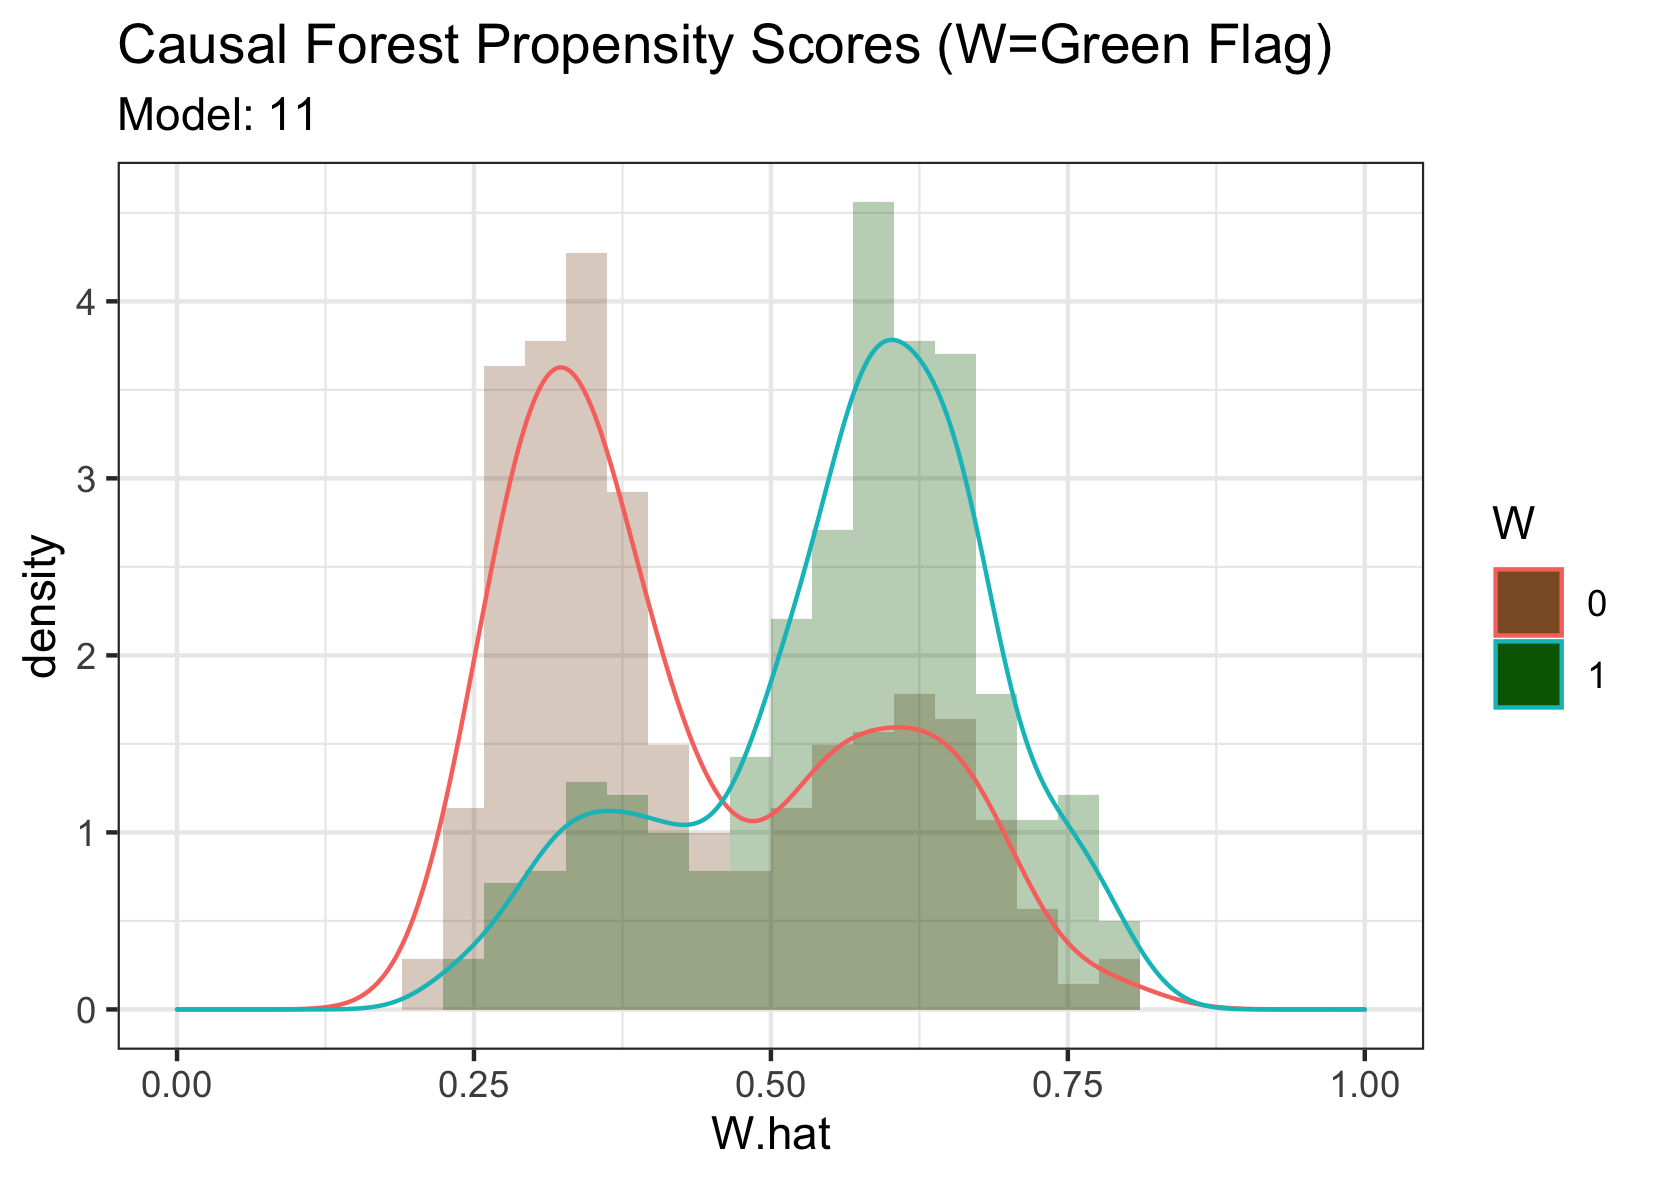
\includegraphics[scale=.15]{chinchilab-template/chapters/appendices/ANALYSIS/prop_11.png}
    \caption{Propensity Score Distribution (Model 11)}
    \label{fig:my_label}
\end{figure}


\begin{table}[H]{
    \begin{subtable}{.5\textwidth}
    \centering
    \footnotesize
        {\begin{tabular}{@{\extracolsep{5pt}}lc} 
        \\[-1.8ex]\hline 
        \hline \\[-1.8ex] 
         & \multicolumn{1}{c}{\textit{Dependent variable: Green Flag}} \\ 
        \cline{2-2} 
        \\[-1.8ex] &   \\ 
        \hline \\[-1.8ex] 
         e.bar & 1.007$^{***}$ \\ 
          & (0.032) \\ 
          & \\ 
         e.residual & 1.403$^{***}$ \\ 
          & (0.100) \\ 
          & \\ 
        \hline \\[-1.8ex] 
        \hline 
        \hline \\[-1.8ex] 
        \textit{Note:}  & \multicolumn{1}{r}{$^{*}$p$<$0.1; $^{**}$p$<$0.05; $^{***}$p$<$0.01} \\ 
        \end{tabular}}
    \subcaption{Outcome Model}
    \end{subtable}
    \begin{subtable}{0.3\linewidth}
    \centering
    \footnotesize
        {\begin{tabular}{@{\extracolsep{5pt}}lc} 
        \\[-1.8ex]\hline 
        \hline \\[-1.8ex] 
         & \multicolumn{1}{c}{\textit{Dependent variable: Green Flag}} \\ 
        \cline{2-2} 
        \\[-1.8ex] &   \\ 
        \hline \\[-1.8ex] 
         m.bar & 0.993$^{***}$ \\ 
          & (0.022) \\ 
          & \\ 
         m.residual & 1.352$^{***}$ \\ 
          & (0.046) \\ 
          & \\ 
        \hline \\[-1.8ex] 
        \hline 
        \hline \\[-1.8ex] 
        \textit{Note:}  & \multicolumn{1}{r}{$^{*}$p$<$0.1; $^{**}$p$<$0.05; $^{***}$p$<$0.01} \\ 
        \end{tabular}}
    \subcaption{Propensity Model}
    \end{subtable}
\caption{Calibration Regressions (Model 11)}
\label{x}}
\end{table}

%%%%%%%%%%%%%%%%%%%%%%%%%%%%%%%%%%%%%%%%%%%%%%%%%%%%%%%%%%%%
\subsubsection{D.2.3.2 Heterogeneity Assessment}
%%%%%%%%%%%%%%%%%%%%%%%%%%%%%%%%%%%%%%%%%%%%%%%%%%%%%%%%%%%%

\begin{table}[h!]
\centering
\caption{Variable Importance (Model 11)}
\begin{tabular}{lr}
\rowcolor[HTML]{FFFFFF} 
\\[-1.8ex]\hline 
\hline \\[-1.8ex] 
{\color[HTML]{333333} \textbf{Covariate}} & {\color[HTML]{333333} \textbf{Value}} \\ \hline
\rowcolor[HTML]{FFFFFF} 
{\color[HTML]{333333} Issue Amount} & \cellcolor[HTML]{00441B}{\color[HTML]{FFFFFF} 0.27828264} \\
\rowcolor[HTML]{FFFFFF} 
{\color[HTML]{333333} Time to Maturity (Days)} & \cellcolor[HTML]{2A924A}{\color[HTML]{FFFFFF} 0.21126808} \\
\rowcolor[HTML]{FFFFFF} 
{\color[HTML]{333333} 2022} & \cellcolor[HTML]{E5F5E0}{\color[HTML]{FFFFFF} 0.06773554} \\
\rowcolor[HTML]{FFFFFF} 
{\color[HTML]{333333} 2017} & \cellcolor[HTML]{EAF7E6}{\color[HTML]{333333} 0.05889331} \\
\rowcolor[HTML]{FFFFFF} 
{\color[HTML]{333333} Financials} & \cellcolor[HTML]{F6FCF4}{\color[HTML]{333333} 0.03908237} \\
\rowcolor[HTML]{FFFFFF} 
{\color[HTML]{333333} 2018} & \cellcolor[HTML]{F7FCF5}{\color[HTML]{333333} 0.03796538} \\ \hline
\end{tabular}
\end{table}

\begin{figure}[h!]
    \centering
    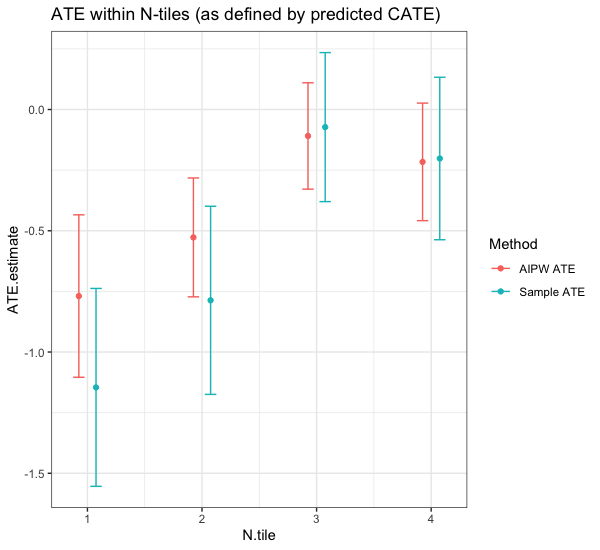
\includegraphics[scale=0.4]{chinchilab-template/chapters/appendices/ANALYSIS/ntile_cf24.png}
    \caption{Graph of ATE within Subgroups (Model 11)}
    \label{fig:my_label}
\end{figure}

\begin{figure}[H]
\centering
   \begin{subfigure}[b]{0.45\textwidth}
    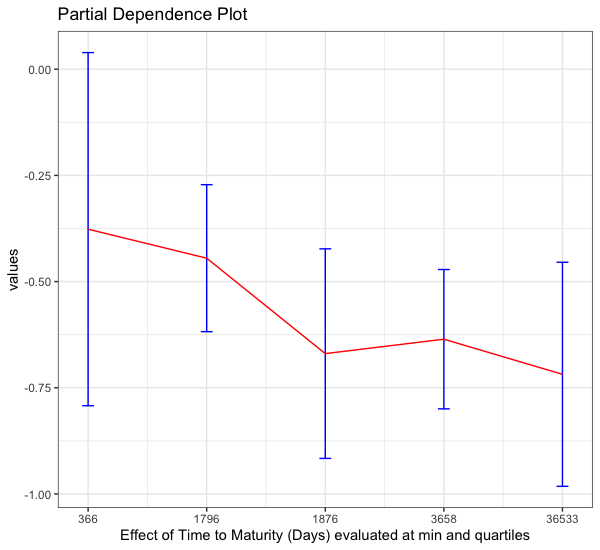
\includegraphics[width=0.8\textwidth]{chinchilab-template/chapters/appendices/ANALYSIS/PDP_cf24.png}
    \caption{Effect of Time to Maturity (Days)}
   \label{fig:Ng1} 
\end{subfigure}
\begin{subfigure}[b]{0.45\textwidth}
    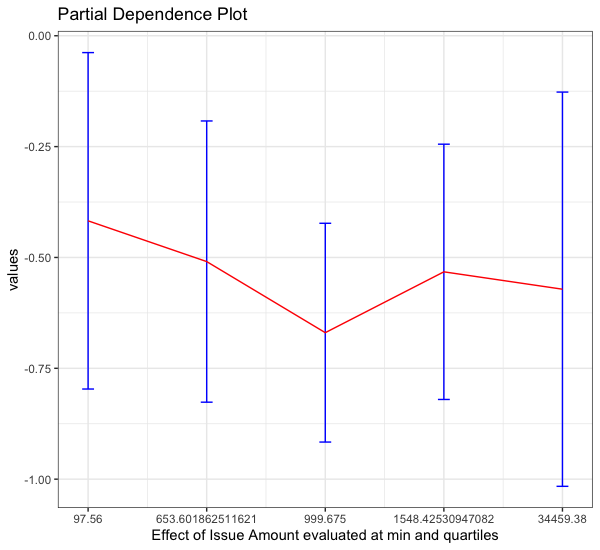
\includegraphics[width=0.8\textwidth]{chinchilab-template/chapters/appendices/ANALYSIS/PDP2_cf24.png}
    \caption{Effect of Issue Amount}
   \label{fig:Ng2}
\end{subfigure}
\\
\begin{subfigure}[b]{0.45\textwidth}
    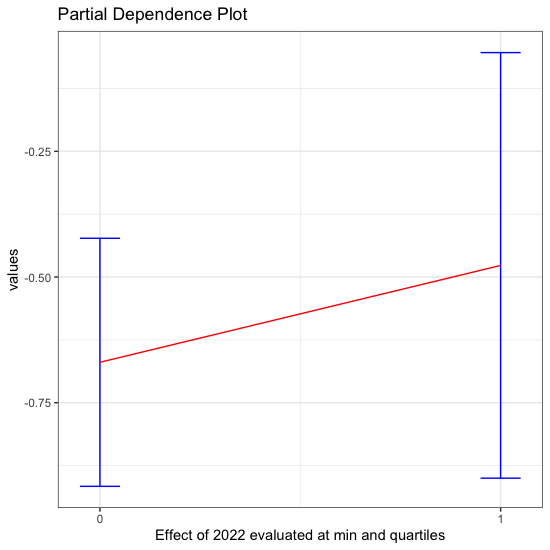
\includegraphics[width=0.8\textwidth]{chinchilab-template/chapters/appendices/ANALYSIS/PDP3_cf24.png}
    \caption{Effect of 2022}
   \label{fig:Ng2}
\end{subfigure}
\caption{Partial Dependency Plots (Model 11)}
\end{figure}


\begin{table}[H]
\caption{Heterogeneity across Covariates (Model 11)}
\label{Het}
\footnotesize
\begin{tabular}{lllll}
\\[-1.8ex]\hline 
\hline \\[-1.8ex] 
{\color[HTML]{333333} \textbf{Variable}} & {\color[HTML]{333333} \textbf{Mean ntile1}} & {\color[HTML]{333333} \textbf{Mean ntile2}} & {\color[HTML]{333333} \textbf{Mean ntile3}} & {\color[HTML]{333333} \textbf{Mean ntile4}} \\
\hline \\[-1.8ex] 
Time to   Maturity (Days) & \cellcolor[HTML]{63BE7B}2931.14 & \cellcolor[HTML]{71C487}2871.15 & \cellcolor[HTML]{71C488}2867.21 & \cellcolor[HTML]{FCFCFF}2227.99 \\
Issue Amount & \cellcolor[HTML]{63BE7B}1439.89 & \cellcolor[HTML]{69C180}1413.98 & \cellcolor[HTML]{78C78D}1346.45 & \cellcolor[HTML]{FCFCFF}730.88 \\
Guarantor & \cellcolor[HTML]{DBEFE2}0.19 & \cellcolor[HTML]{D5EDDE}0.22 & \cellcolor[HTML]{D9EEE1}0.2 & \cellcolor[HTML]{EEF7F3}0.08 \\
2013 & \cellcolor[HTML]{EBF5F0}0.1 & \cellcolor[HTML]{F4F9F8}0.05 & \cellcolor[HTML]{F9FBFC}0.02 & \cellcolor[HTML]{FBFCFE}0.01 \\
2014 & \cellcolor[HTML]{EBF5F0}0.1 & \cellcolor[HTML]{F5FAF9}0.04 & \cellcolor[HTML]{F9FBFC}0.02 & \cellcolor[HTML]{FCFCFF}0 \\
2015 & \cellcolor[HTML]{F4F9F8}0.05 & \cellcolor[HTML]{EEF7F3}0.08 & \cellcolor[HTML]{EEF7F3}0.08 & \cellcolor[HTML]{F0F7F5}0.07 \\
2016 & \cellcolor[HTML]{EEF7F3}0.08 & \cellcolor[HTML]{E9F5EF}0.11 & \cellcolor[HTML]{EBF5F0}0.1 & \cellcolor[HTML]{F4F9F8}0.05 \\
2017 & \cellcolor[HTML]{FCFCFF}0 & \cellcolor[HTML]{FCFCFF}0 & \cellcolor[HTML]{EBF5F0}0.1 & \cellcolor[HTML]{C9E8D3}0.29 \\
2018 & \cellcolor[HTML]{FCFCFF}0 & \cellcolor[HTML]{F5FAF9}0.04 & \cellcolor[HTML]{E2F2E8}0.15 & \cellcolor[HTML]{D9EEE1}0.2 \\
2019 & \cellcolor[HTML]{E9F5EF}0.11 & \cellcolor[HTML]{DEF0E5}0.17 & \cellcolor[HTML]{E5F3EC}0.13 & \cellcolor[HTML]{E5F3EC}0.13 \\
2020 & \cellcolor[HTML]{E9F5EF}0.11 & \cellcolor[HTML]{ECF6F2}0.09 & \cellcolor[HTML]{EEF7F3}0.08 & \cellcolor[HTML]{F7FAFB}0.03 \\
2021 & \cellcolor[HTML]{DEF0E5}0.17 & \cellcolor[HTML]{E2F2E8}0.15 & \cellcolor[HTML]{E7F4ED}0.12 & \cellcolor[HTML]{F9FBFC}0.02 \\
2022 & \cellcolor[HTML]{FCFCFF}0 & \cellcolor[HTML]{E9F5EF}0.11 & \cellcolor[HTML]{E4F2EA}0.14 & \cellcolor[HTML]{DBEFE2}0.19 \\
Annual Coupon & \cellcolor[HTML]{77C68C}0.75 & \cellcolor[HTML]{8CCF9F}0.63 & \cellcolor[HTML]{89CE9C}0.65 & \cellcolor[HTML]{67C07F}0.84 \\
Semi Annual   Coupon & \cellcolor[HTML]{D0EAD9}0.25 & \cellcolor[HTML]{BBE2C7}0.37 & \cellcolor[HTML]{BEE3CA}0.35 & \cellcolor[HTML]{E0F1E7}0.16 \\
Quarterly & \cellcolor[HTML]{FCFCFF}0 & \cellcolor[HTML]{FCFCFF}0 & \cellcolor[HTML]{FCFCFF}0 & \cellcolor[HTML]{FCFCFF}0 \\
Senior   Secured Mortgage & \cellcolor[HTML]{EEF7F3}0.08 & \cellcolor[HTML]{EBF5F0}0.1 & \cellcolor[HTML]{EEF7F3}0.08 & \cellcolor[HTML]{E2F2E8}0.15 \\
Senior Secured & \cellcolor[HTML]{F7FAFB}0.03 & \cellcolor[HTML]{FBFCFE}0.01 & \cellcolor[HTML]{F7FAFB}0.03 & \cellcolor[HTML]{F9FBFC}0.02 \\
Senior Unsecured & \cellcolor[HTML]{72C488}0.78 & \cellcolor[HTML]{7CC991}0.72 & \cellcolor[HTML]{85CC99}0.67 & \cellcolor[HTML]{ACDCBA}0.45 \\
Senior Non   Preferred & \cellcolor[HTML]{FBFCFE}0.01 & \cellcolor[HTML]{F2F8F6}0.06 & \cellcolor[HTML]{ECF6F2}0.09 & \cellcolor[HTML]{E9F5EF}0.11 \\
Senior Preferred & \cellcolor[HTML]{FCFCFF}0 & \cellcolor[HTML]{F4F9F8}0.05 & \cellcolor[HTML]{EEF7F3}0.08 & \cellcolor[HTML]{D2EBDB}0.24 \\
Senior   Subordinated Unsecured & \cellcolor[HTML]{FCFCFF}0 & \cellcolor[HTML]{FCFCFF}0 & \cellcolor[HTML]{FCFCFF}0 & \cellcolor[HTML]{FCFCFF}0 \\
Subordinated   Unsecured & \cellcolor[HTML]{FBFCFE}0.01 & \cellcolor[HTML]{FCFCFF}0 & \cellcolor[HTML]{FBFCFE}0.01 & \cellcolor[HTML]{FCFCFF}0 \\
Basic Materials & \cellcolor[HTML]{FCFCFF}0 & \cellcolor[HTML]{F9FBFC}0.02 & \cellcolor[HTML]{FCFCFF}0 & \cellcolor[HTML]{FCFCFF}0 \\
Consumer   Cyclicals & \cellcolor[HTML]{FBFCFE}0.01 & \cellcolor[HTML]{FBFCFE}0.01 & \cellcolor[HTML]{FCFCFF}0 & \cellcolor[HTML]{FCFCFF}0 \\
Consumer   Non Cyclicals & \cellcolor[HTML]{FBFCFE}0.01 & \cellcolor[HTML]{F9FBFC}0.02 & \cellcolor[HTML]{FCFCFF}0 & \cellcolor[HTML]{FCFCFF}0 \\
Financials & \cellcolor[HTML]{9BD5AB}0.55 & \cellcolor[HTML]{95D3A6}0.58 & \cellcolor[HTML]{85CC99}0.67 & \cellcolor[HTML]{63BE7B}0.86 \\
Healthcare & \cellcolor[HTML]{FCFCFF}0 & \cellcolor[HTML]{FCFCFF}0 & \cellcolor[HTML]{FCFCFF}0 & \cellcolor[HTML]{FCFCFF}0 \\
Industrials & \cellcolor[HTML]{F5FAF9}0.04 & \cellcolor[HTML]{F7FAFB}0.03 & \cellcolor[HTML]{F5FAF9}0.04 & \cellcolor[HTML]{F7FAFB}0.03 \\
Institutions,   Associations \& Organizations & \cellcolor[HTML]{F5FAF9}0.04 & \cellcolor[HTML]{F2F8F6}0.06 & \cellcolor[HTML]{F5FAF9}0.04 & \cellcolor[HTML]{F9FBFC}0.02 \\
Real Estate & \cellcolor[HTML]{FCFCFF}0 & \cellcolor[HTML]{F9FBFC}0.02 & \cellcolor[HTML]{FCFCFF}0 & \cellcolor[HTML]{FCFCFF}0 \\
Technology & \cellcolor[HTML]{FBFCFE}0.01 & \cellcolor[HTML]{FBFCFE}0.01 & \cellcolor[HTML]{FCFCFF}0 & \cellcolor[HTML]{FCFCFF}0 \\
Utilities & \cellcolor[HTML]{ECF6F2}0.09 & \cellcolor[HTML]{F5FAF9}0.04 & \cellcolor[HTML]{F4F9F8}0.05 & \cellcolor[HTML]{FBFCFE}0.01 \\
AAA & \cellcolor[HTML]{B0DDBD}0.43 & \cellcolor[HTML]{BBE2C7}0.37 & \cellcolor[HTML]{BEE3CA}0.35 & \cellcolor[HTML]{CEEAD8}0.26 \\
AA & \cellcolor[HTML]{E5F3EC}0.13 & \cellcolor[HTML]{D9EEE1}0.2 & \cellcolor[HTML]{D7EDDF}0.21 & \cellcolor[HTML]{CBE8D5}0.28 \\
A & \cellcolor[HTML]{DBEFE2}0.19 & \cellcolor[HTML]{D7EDDF}0.21 & \cellcolor[HTML]{DCF0E4}0.18 & \cellcolor[HTML]{CBE8D5}0.28 \\
BBB & \cellcolor[HTML]{D2EBDB}0.24 & \cellcolor[HTML]{D7EDDF}0.21 & \cellcolor[HTML]{D0EAD9}0.25 & \cellcolor[HTML]{DBEFE2}0.19 \\
BB & \cellcolor[HTML]{FBFCFE}0.01 & \cellcolor[HTML]{F9FBFC}0.02 & \cellcolor[HTML]{FBFCFE}0.01 & \cellcolor[HTML]{FCFCFF}0 \\
AUD & \cellcolor[HTML]{FCFCFF}0 & \cellcolor[HTML]{FCFCFF}0 & \cellcolor[HTML]{FBFCFE}0.01 & \cellcolor[HTML]{FCFCFF}0 \\
CAD & \cellcolor[HTML]{F9FBFC}0.02 & \cellcolor[HTML]{F7FAFB}0.03 & \cellcolor[HTML]{F9FBFC}0.02 & \cellcolor[HTML]{FBFCFE}0.01 \\
CLP & \cellcolor[HTML]{FCFCFF}0 & \cellcolor[HTML]{FCFCFF}0 & \cellcolor[HTML]{FCFCFF}0 & \cellcolor[HTML]{FCFCFF}0 \\
CNY & \cellcolor[HTML]{FCFCFF}0 & \cellcolor[HTML]{FCFCFF}0 & \cellcolor[HTML]{FCFCFF}0 & \cellcolor[HTML]{FCFCFF}0 \\
EUR & \cellcolor[HTML]{85CC99}0.67 & \cellcolor[HTML]{97D3A8}0.57 & \cellcolor[HTML]{92D1A3}0.6 & \cellcolor[HTML]{6BC182}0.82 \\
GBP & \cellcolor[HTML]{F5FAF9}0.04 & \cellcolor[HTML]{F9FBFC}0.02 & \cellcolor[HTML]{FBFCFE}0.01 & \cellcolor[HTML]{FCFCFF}0 \\
JPY & \cellcolor[HTML]{FBFCFE}0.01 & \cellcolor[HTML]{FCFCFF}0 & \cellcolor[HTML]{FCFCFF}0 & \cellcolor[HTML]{FCFCFF}0 \\
NZD & \cellcolor[HTML]{FCFCFF}0 & \cellcolor[HTML]{FCFCFF}0 & \cellcolor[HTML]{FCFCFF}0 & \cellcolor[HTML]{FCFCFF}0 \\
NOK & \cellcolor[HTML]{FCFCFF}0 & \cellcolor[HTML]{FCFCFF}0 & \cellcolor[HTML]{FCFCFF}0 & \cellcolor[HTML]{FCFCFF}0 \\
SEK & \cellcolor[HTML]{F9FBFC}0.02 & \cellcolor[HTML]{FCFCFF}0 & \cellcolor[HTML]{FCFCFF}0 & \cellcolor[HTML]{FCFCFF}0 \\
\hline \\[-1.8ex] 
\end{tabular}
\end{table}

